\documentclass{article}

\usepackage[utf8]{vietnam}
\usepackage{amsmath}
\usepackage{graphicx}
\usepackage{setspace}
\usepackage{fancyhdr}
\usepackage[left=3.5cm,right=2cm,top=3.5cm,bottom=3cm]{geometry}
\usepackage{titlesec}
\usepackage{placeins}
\usepackage{multirow}
\usepackage{multicol}
\usepackage{caption}
\usepackage{amsfonts}
\usepackage{amssymb}

\titleformat{\section}
  {\normalfont\fontsize{14}{20}\bfseries}{\thesection}{1em}{}

\titleformat{\subsection}
  {\normalfont\fontsize{14}{20}\bfseries}{\thesubsection}{1em}{}
  
\titleformat{\subsubsection}
  {\normalfont\fontsize{14}{20}\bfseries}{\thesubsubsection}{1em}{}
  
\makeatletter
\renewcommand{\tableofcontents}{%
  \@starttoc{toc}%
}
\makeatother

\begin{document}
%------------------------------------------------------------
%|						COVER PAGE							|
%------------------------------------------------------------
\begin{center}
	\pagenumbering{gobble}
	\fontsize{14}{20}\selectfont
	\textsc{TỔNG LIÊN ĐOÀN LAO ĐỘNG VIỆT NAM\\ 
	\textbf{TRƯỜNG ĐẠI HỌC TÔN ĐỨC THẮNG\\} 
	\textbf{KHOA CÔNG NGHỆ THÔNG TIN}}
	
	\vspace{0.8cm}
	\begin{figure}[htp]
	\begin{center}
		
\includegraphics[scale=0.04]{images/logo.png}
	\end{center}
	\end{figure}

	\fontsize{16}{20}\selectfont\textbf{ĐỒ ÁN MÔN HỆ THỐNG THƯƠNG MẠI THÔNG MINH\\}
	
	\vspace{2cm}
	\fontsize{24}{20}\selectfont\textbf{DỰ BÁO THỜI TIẾT KHÍ HẬU VÀ LƯU LƯỢNG MƯA Ở AUSTRALIA}
\end{center}

\vspace{1cm}
\begin{flushright}
	\setstretch{1.5}
	\fontsize{14}{20}\selectfont
	\textit{Người hướng dẫn}: \textbf{TS DƯƠNG HỮU PHÚC}\\
	\textit{Người thực hiện}: \textbf{NGUYỄN HOÀNG TRÚC – 51800319}\\
	\textbf{PHÙ Ý KỲ - 51800989}\\
	\textbf{NGUYỄN VĂN ĐIỂM - 51900310}\\
	\textit{Lớp}: \textbf{18050402 - 19050302}\\
	\textit{Khóa}: \textbf{22-23}\\
\end{flushright}

\vspace{1cm}
\begin{center}
	\fontsize{14}{20}\selectfont
	\textbf{THÀNH PHỐ HỒ CHÍ MINH, NĂM 2021}
\end{center}
\pagebreak

%------------------------------------------------------------
%|						TITLE PAGE							|
%------------------------------------------------------------
\begin{center}
	\pagenumbering{gobble}
	\fontsize{14}{20}\selectfont
	\textsc{TỔNG LIÊN ĐOÀN LAO ĐỘNG VIỆT NAM\\ 
	\textbf{TRƯỜNG ĐẠI HỌC TÔN ĐỨC THẮNG\\} 
	\textbf{KHOA CÔNG NGHỆ THÔNG TIN}}
	
	\vspace{0.8cm}
	\begin{figure}[htp]
	\begin{center}
		
\includegraphics[scale=0.04]{images/logo.png}
	\end{center}
	\end{figure}

	\fontsize{16}{20}\selectfont\textbf{ĐỒ ÁN MÔN HỆ THỐNG THƯƠNG MẠI THÔNG MINH\\}
	
	\vspace{2cm}
	\fontsize{24}{20}\selectfont\textbf{DỰ BÁO THỜI TIẾT KHÍ HẬU VÀ LƯU LƯỢNG MƯA Ở AUSTRALIA}
\end{center}

\vspace{1cm}
\begin{flushright}
	\setstretch{1.5}
	\fontsize{14}{20}\selectfont
	\textit{Người hướng dẫn}: \textbf{TS DƯƠNG HỮU PHÚC}\\
	\textit{Người thực hiện}: \textbf{NGUYỄN HOÀNG TRÚC – 51800319}\\
	\textbf{PHÙ Ý KỲ - 51800989}\\
	\textbf{NGUYỄN VĂN ĐIỂM - 51900310}\\
	\textit{Lớp}: \textbf{18050402 - 19050302}\\
	\textit{Khóa}: \textbf{22-23}\\
\end{flushright}

\vspace{1cm}
\begin{center}
	\fontsize{14}{20}\selectfont
	\textbf{THÀNH PHỐ HỒ CHÍ MINH, NĂM 2021}
\end{center}
\pagebreak

%------------------------------------------------------------
%|							PAGE i							|
%------------------------------------------------------------
\pagestyle{fancy}
\fancyhf{}
\chead{\thepage}
\renewcommand{\headrulewidth}{0pt}
\begin{center}
	\pagenumbering{roman}\setcounter{page}{1}
	\fontsize{16}{20}\selectfont
	\textbf{LỜI CẢM ƠN\\} 
\end{center}
\addcontentsline{toc}{section}{LỜI CẢM ƠN}
	\setstretch{1.5}
	\fontsize{13}{13}\selectfont
	\paragraph{}
	Trong quá trình học tập và nghiên cứu đề tài “Tìm hiểu phân tích Australia ngày tiếp theo liệu có mưa” chúng em nhận được sự giúp đỡ và hướng dẫn của Thầy Dương Hữu Phúc, để hoàn thành bài đồ án này. Chúng em xin cảm ơn và bảy tỏ lòng biết ơn với Ban giám hiệu nhà trường Đại học Tôn Đức Thắng, khoa Công nghệ thông tin, các thầy cô giáo đã tham gia quản lý, giảng dạy và giúp đỡ em trong suốt thời gian học tập môn Hệ thống thương mại thông minh.
	Chúng em xin bày tỏ lòng biết ơn sâu sắc đến Thầy Dương Hữu Phúc – Người đã trực tiếp giảng dạy môn môn Hệ thống thương mại thông minh. Chúng em xin cảm ơn bạn bè, thầy cô đã hỗ trợ và giúp đỡ chúng em trong quá trình học tập.
 
\pagebreak	%------------------------------------------------------------
%|							PAGE ii							|
%------------------------------------------------------------
\begin{center}
	\setstretch{1.0}
	\fontsize{16}{20}\selectfont
	\textbf{ĐỒ ÁN ĐƯỢC HOÀN THÀNH}\\
	\textbf{TẠI TRƯỜNG ĐẠI HỌC TÔN ĐỨC THẮNG\\} 
\end{center}
	\setstretch{1.5}
	\fontsize{13}{13}\selectfont
	\paragraph{}
	Tôi xin cam đoan đây là sản phẩm đồ án của riêng chúng tôi và được sự hướng dẫn của thầy Dương Hữu Phúc. Các nội dung nghiên cứu, kết quả trong đề tài này là trung thực và chưa công bố dưới bất kỳ hình thức nào trước đây. Những số liệu trong các bảng biểu phục vụ cho việc phân tích, nhận xét, đánh giá được chính tác giả thu thập từ các nguồn khác nhau có ghi rõ trong phần tài liệu tham khảo.	
	\paragraph{}
	Ngoài ra, trong đồ án còn sử dụng một số nhận xét, đánh giá cũng như số liệu của các tác giả khác, cơ quan tổ chức khác đều có trích dẫn và chú thích nguồn gốc.
	\paragraph{}
	\textbf{Nếu phát hiện có bất kỳ sự gian lận nào chúng tôi xin hoàn toàn chịu trách nhiệm về nội dung đồ án của mình.} Trường đại học Tôn Đức Thắng không liên quan đến những vi phạm tác quyền, bản quyền do tôi gây ra trong quá trình thực hiện (nếu có).
\begin{flushright}
	TP. Hồ Chí Minh,  ngày   tháng   năm   \\ 
	\textit{Tác giả\\
	(ký tên và ghi rõ họ tên)\\
	\vspace{1.5cm}
	Nguyễn Hoàng Trúc\\
	\vspace{1.5cm}
	Phù Ý Kỳ\\
	\vspace{1.5cm}
	Nguyễn Văn Điểm\\}
\end{flushright}
\pagebreak

%------------------------------------------------------------
%|						PAGE iii							|
%------------------------------------------------------------
\begin{center}
	\setstretch{1.0}
	\fontsize{16}{20}\selectfont
	\textbf{PHẦN XÁC NHẬN VÀ ĐÁNH GIÁ CỦA GIẢNG VIÊN}\\
\end{center}
\addcontentsline{toc}{section}{PHẦN XÁC NHẬN VÀ ĐÁNH GIÁ CỦA GIẢNG VIÊN}
\setstretch{1.5}
\fontsize{13}{13}\selectfont
\textbf{Phần xác nhận của GV hướng dẫn}\\
................................................................................................................................\\
................................................................................................................................\\
................................................................................................................................\\
................................................................................................................................\\
................................................................................................................................\\
\begin{flushright}
	TP. Hồ Chí Minh,  ngày   tháng   năm   \\ 
	(ký tên và ghi rõ họ tên)\\
	\vspace{3cm}
\end{flushright}
\setstretch{1.5}
\fontsize{13}{13}\selectfont
\textbf{Phần đánh giá của GV chấm bài}\\
................................................................................................................................\\
................................................................................................................................\\
................................................................................................................................\\
................................................................................................................................\\
................................................................................................................................\\
\begin{flushright}
	TP. Hồ Chí Minh,  ngày   tháng   năm   \\ 
	(ký tên và ghi rõ họ tên)\\
	\vspace{3cm}
\end{flushright}
\pagebreak

%------------------------------------------------------------
%|							PAGE iv							|
%------------------------------------------------------------
\begin{center}
	\fontsize{16}{20}\selectfont
	\textbf{TÓM TẮT\\} 
\end{center}
\addcontentsline{toc}{section}{TÓM TẮT}
	\setstretch{1.5}
	\fontsize{13}{13}\selectfont
	\paragraph{}
	Trong bày báo cáo này gồm có 4 chương:
	\paragraph{}Chương 1 nói về tổng quan đề tài, giới thiệu đề tài và phương pháp nghiên cứu với ứng dụng thực tế của đề tài. Dựa vào data weatherAUS.csv được thu thập trong thực tế  từ kaggle.com trong Rain in Australia để dự đoán xác suất ngày tiếp theo ở Australia có mưa không. Tiến hành xử lý missing value, tiến hành phân tích data set bằng cách train và test, áp dụng lý thuyết và thực thi đề tài bằng thuật toán hồi quy Logistic (Logistic Regression), thuật toán Machine Learning rừng ngẫu nhiên (Random Forest Machine Learning), thuật toán Naive Bayes và thuật toán XGBoost, trực quan hóa dữ liệu, đánh giá đo lường và cho ra kết quả.
	\paragraph{}Chương 2 tổng quan giải thuật cơ sở lý thuyết của các thuật toán đề áp dụng vào dataset dự báo thời tiết bao gồm các thuật toán  hồi quy Logistic (Logistic Regression), thuật toán Machine Learning rừng ngẫu nhiên (Random Forest Machine Learning), thuật toán Naive Bayes và thuật toán XGBoost. Mỗi thuật toán sẽ được nêu lý thuyết liên quan và ưu nhược điểm của từng thuật toán, khi áp dụng vào dataset dự báo thời tiết thì sẽ áp dụng những gì.
	\paragraph{}Chương 3 thực nghiệm bao gồm đặt tả dataset nêu ra cụ thể từng thuộc tính có tác dụng gì, các yếu tố ảnh hưởng đến dự đoán mưa vào ngày mai, thực hiện hóa bằng dồ thị tableau và code bằng ngôn ngữ python demo dataset dự đoán xác suất. Khi cho ra được kết quả dự đoán sẽ so sánh được thuật toán nào tối ưu hơn khi áp dụng dataset dự báo thời tiết ở nước Úc
	\paragraph{}Chương 4 kết luận những điều đã đạt được trong báo cáo, tóm tắt các ý chính trong báo cáo, định hướng nghiên cứu trong tương lai.
\pagebreak

%------------------------------------------------------------
%|					TABLEOFCONTENT PAGE						|
%------------------------------------------------------------
\pagenumbering{arabic}\setcounter{page}{1}
\begin{center}
	\fontsize{16}{20}\selectfont
	\textbf{MỤC LỤC\\}
\end{center}
\addcontentsline{toc}{section}{MỤC LỤC}
\tableofcontents
\pagebreak

%------------------------------------------------------------
%|			LISTOFGRAPHICS AND LISTOFTABLES PAGE			|
%------------------------------------------------------------
\begin{center}
	\fontsize{16}{20}\selectfont
	\textbf{DANH MỤC CÁC BẢNG BIỂU, HÌNH VẼ, ĐỒ THỊ}
\end{center}
\addcontentsline{toc}{section}{DANH MỤC CÁC BẢNG BIỂU, HÌNH VẼ, ĐỒ THỊ}
\listoffigures
\listoftables
\pagebreak

%------------------------------------------------------------
%|					CONTENT PAGES							|
%------------------------------------------------------------
\section*{CHƯƠNG 1 - TỔNG QUAN ĐỀ TÀI}
\addcontentsline{toc}{section}{CHƯƠNG 1 - TỔNG QUAN ĐỀ TÀI}
\setcounter{section}{1}

\subsection{Giới thiệu đề tài}
\paragraph{}


\begin{figure}[!h]
	\begin{center}
		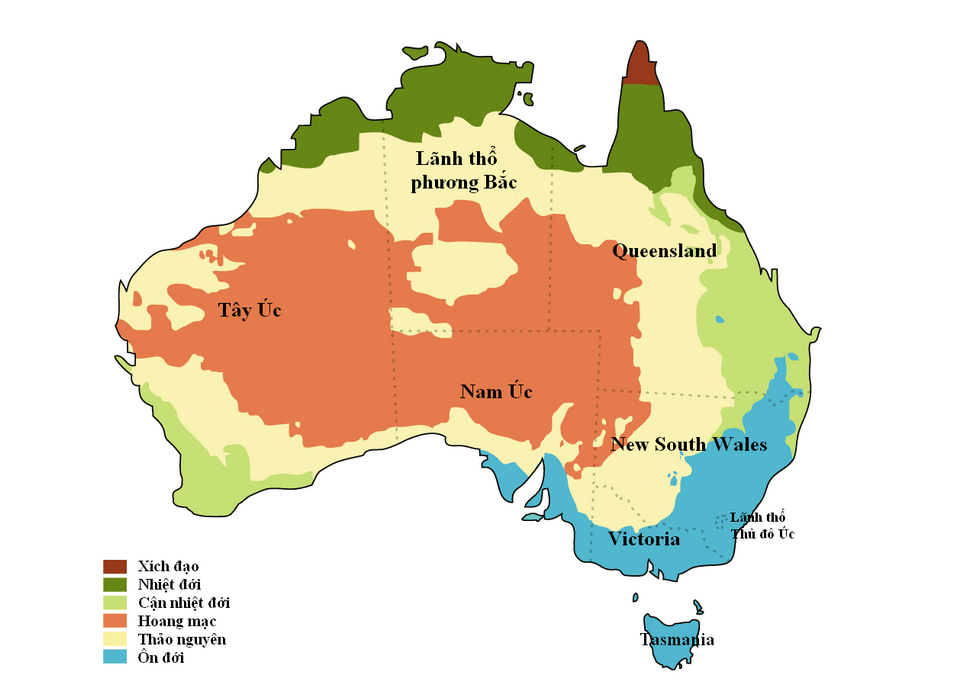
\includegraphics[width=\linewidth]{images/Bando.png}
		\caption{\fontsize{14}{20}\selectfont Bản đồ}
         (Nguồn:https://hchuman.com/thoi-tiet-nuoc-uc-khi-hau-4-mua-khac-la-o-cac-bang-cua-uc.html)
	\end{center}
\end{figure}
\pagebreak
\paragraph{}
Nước Úc là nơi đa dạng về khí hậu. Để hiểu rõ nguyên nhân gây nên sự khác biệt của thời tiết nước Úc, chúng ta hãy quay về địa lý. Châu Úc nằm ở bán cầu Nam, đối lập thời tiết hoàn toàn với những nước ở bàn cầu Bắc. Khi ở bán cầu Bắc là mùa đông thì ở Úc là mùa hè ấm áp và ngược lại khi Úc chìm trong băng giá tháng 6 thì ở bán cầu Bắc đang là mùa hè rực rỡ.
\paragraph{}
 Để thực hiên chính xác thì “Dự báo thời tiết” đã ra đời. Dự báo thời tiết là một trong những những nhu cầu thiết yếu mà con người vô cùng quan tâm và chú trọng bởi nó ảnh hưởng tới cuộc sống và kinh tế phát triển của quốc gia.
\subsection{Phát biểu bài toán}
\paragraph{}Ngày nay vấn đề dự đoán thời tiết đã có vô số lời giải, có rất nhiều thuật toán được áp dụng trong lĩnh vực phân tích cho dự báo thời tiết hiệu quả bao gồm thuật toán hồi quy Logistic (Logistic Regression), thuật toán Machine Learning rừng ngẫu nhiên (Random Forest Machine Learning), thuật toán Naive Bayes và thuật toán XGBoost,...
\paragraph{}Một trong những thuật toán được áp dụng trong lĩnh vực phân tích cho dự báo thời tiết hiệu quả nhất đó là Logistic Regression. Hồi quy logistic (Logistic Regression) là một mô hình thống kê, mô hình hoá biến phụ thuộc nhị phân. Về cơ bản, Logistic Regression là tìm mối quan hệ giữa các đặc trưng và xác suất của kết quả cụ thể (0 hoặc 1, yes hoặc no,..).
\paragraph{}
  
\subsection{Mục tiêu đề tài}
\paragraph{}
Dựa vào data weatherAUS.csv được được thu thập trong thực tế  từ kaggle.com trong Rain in Australia để dự đoán dự đoán xác suất ngày tiếp theo ở Australia có mưa không.
	
\subsection{Phạm vi đề tài}
\paragraph{}
Nước Úc là một quốc gia bao gồm một đảo lớn là Tasmania, một tiểu bang của Úc và nhiều hòn đảo nhỏ ở Thái Bình Dương và Ấn Độ Dương. Với diện tích đất gần 7,7 triệu km2 và là quốc gia lớn thứ sáu về diện tích trên thế giới.
\paragraph{}
	Dữ liệu có liên quan trực tiếp đến dự báo thời tiết của một quốc gia. Dữ liệu weatherAUS.csv được nghiên cứu bao gồm: Nhiệt độ, lượng mưa, độ bốc hơi, độ ẩm, áp xuất, hướng gió, vận tốc gió và mật độ mây được thu thập trong 10 năm (từ 1/12/2008 đến 25/6/2017) ở 49 trạm khí tượng của nước Úc.
    \begin{figure}[!h]
	\begin{center}
		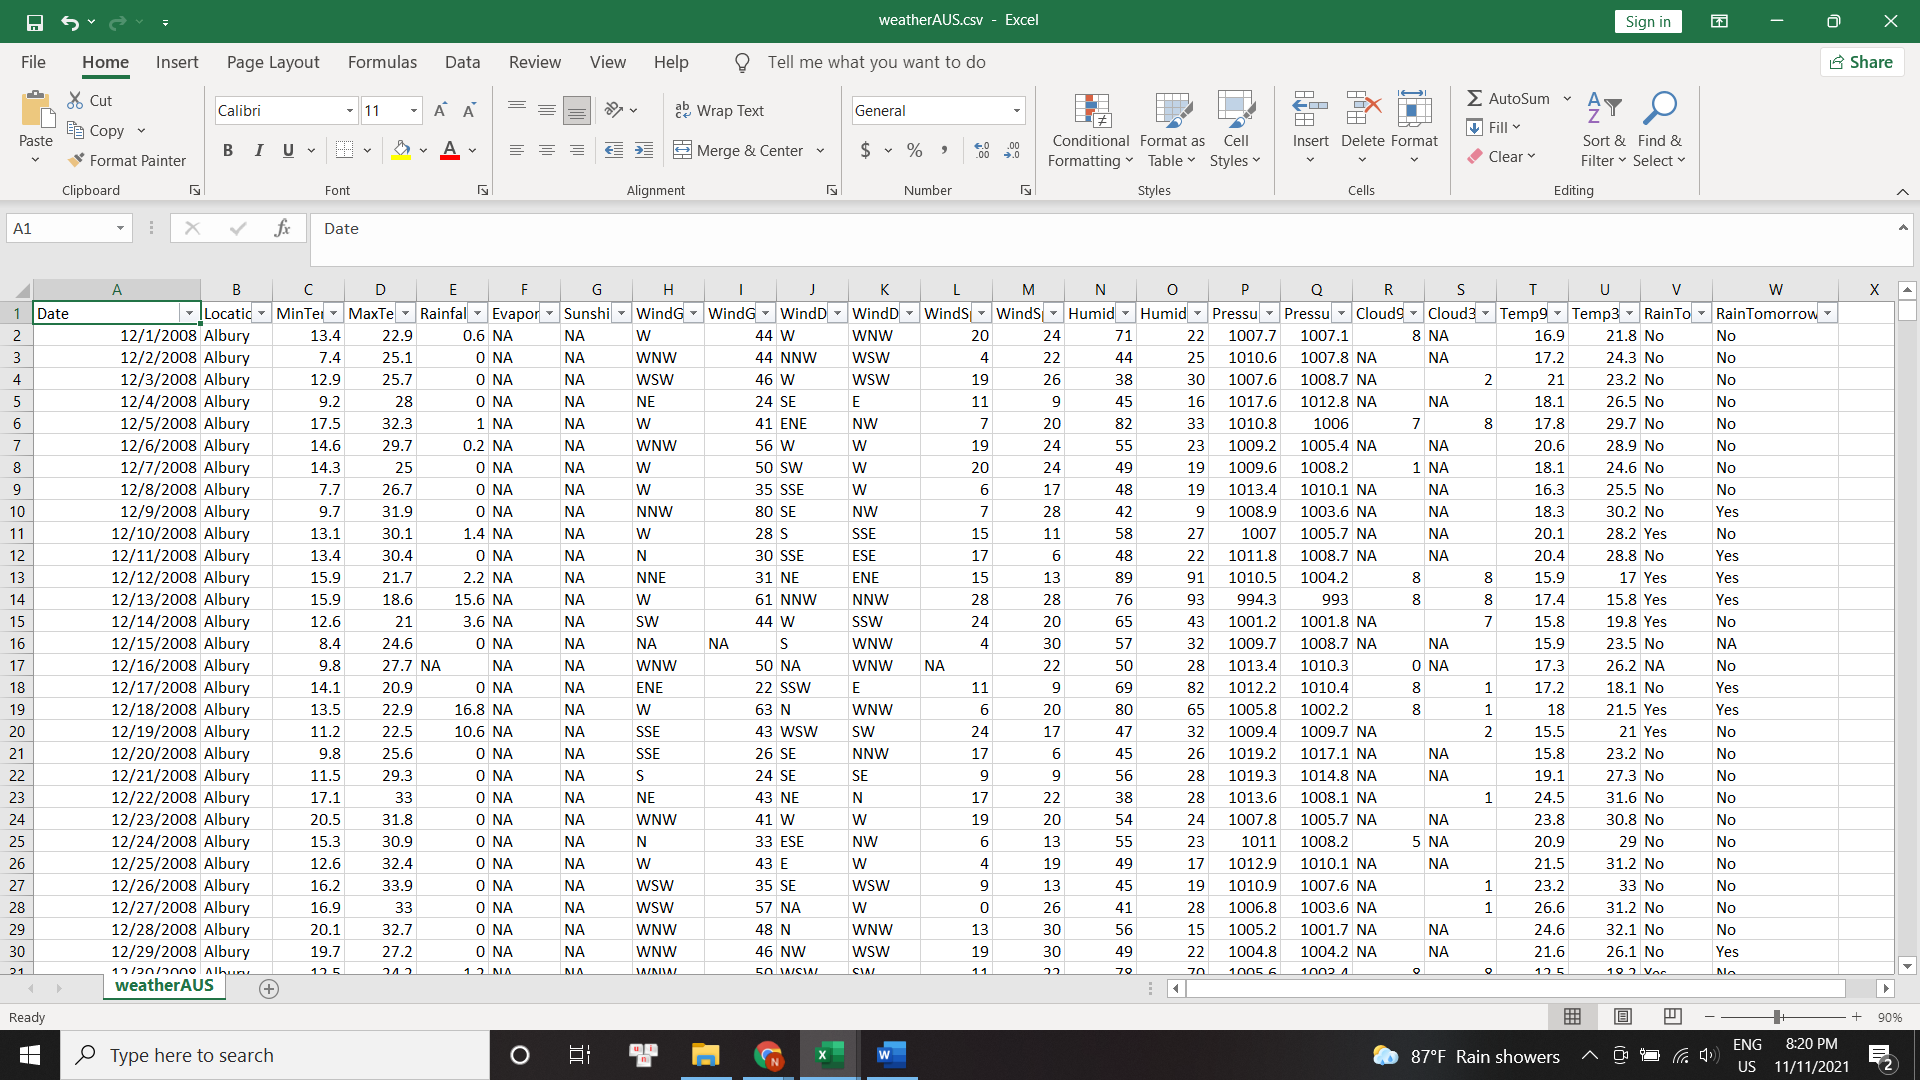
\includegraphics[width=\linewidth]{images/dataset.png}
		\caption{\fontsize{14}{20}\selectfont Dataset thời tiết ở Úc}      
	\end{center}
\end{figure}
\paragraph{}
    Link dataset: https://www.kaggle.com/jsphyg/weather-dataset-rattle-package

\subsection{Phương pháp nghiên cứu}
\paragraph{}Tiến hành xử lý missing value.
\paragraph{}Tiến hành phân tích data set theo phương pháp hold-out bằng cách chia tập dữ liệu thành 2 phần data train và test.
\paragraph{} Áp dụng lý thuyết và thực thi đề tài bằng thuật toán hồi quy Logistic, thuật toán Machine Learning rừng ngẫu nhiên (Random Forest Machine Learning), thuật toán Naive Bayes và thuật toán XGBoost.
\paragraph{} Trực quan hóa dữ liệu, đánh giá đo lường và cho ra kết quả.

\subsection{Ý nghĩa khoa học và thực tiễn}
  \paragraph{}Dự báo thời tiết ở Úc giúp cho cá nhân, tổ chức lên kế hoạch vào ngày tiếp theo từ đó phát triển những thuận lợi mà dự báo thời tiết mang đến. 
  \paragraph{}  
  Việc dự đoán trước thời tiết như vậy có ảnh hưởng lớn đến nhiều ngành nghề trong một quốc gia mà còn là nhu cầu thiết yếu hằng ngày của quốc gia đó.
  \paragraph{}
  Việc đơn giản giản khi dự báo thời tiết ngày mai có mưa không ảnh hưởng đến đời sống cá nhân như là phải chuẩn bị ô dù, áo mưa,....
   \paragraph{} Người làm nông nghiệp, dịch vụ, sản xuất...
   \paragraph{}Giúp cho những người làm khí tượng có thể dự đoán để đưa ra các cảnh báo và giải pháp cho người dân sống tốt hơn.
\pagebreak

\section*{CHƯƠNG 2 - TỔNG QUAN GIẢI THUẬT}
\addcontentsline{toc}{section}{CHƯƠNG 2 - TỔNG QUAN GIẢI THUẬT}
\setcounter{section}{2}
\setcounter{subsection}{0}

\subsection{Giới thiệu về hồi quy logistic (Logistic Regression)}
\paragraph{}
 Trong thực tế, hồi quy logistic dùng để dự đoán xác suất xảy ra của một vấn đề cụ thể. Trong dự báo thời tiết, hồi quy logistic không chỉ dự đoán một ngày trong tương lai có mưa hay không, mà còn dự đoán được xác suất xảy ra mưa. Tương tự, hồi quy logistic có thể được sử dụng để dự đoán khả năng bệnh nhân mắc một bệnh cụ thể với các triệu chứng nhất định, đó là lý do tại sao nó rất phổ biến trong lĩnh vực y học.
\paragraph{}
Hồi quy logistic là một kỹ thuật thống kê được giám sát để tìm xác suất của biến phụ thuộc (Các lớp có trong biến).
\paragraph{}
Hồi quy logistic sử dụng các hàm được gọi là hàm logit, giúp suy ra mối quan hệ giữa biến phụ thuộc và các biến độc lập bằng cách dự đoán xác suất hoặc cơ hội xảy ra.
\paragraph{}
Các hàm logistic (còn được gọi là hàm sigmoid) chuyển đổi xác suất thành các giá trị nhị phân có thể được sử dụng thêm cho các dự đoán.
 \paragraph{}
 Logistic regression được áp dụng trong bài toán phân loại nhị phân (Binary classification) tức ta sẽ có hai output, hoặc có thể gọi là hai nhãn (ví dụ như 0 và 1 hoặc Yes or No).
	
\subsubsection{Trong thống kê}
\paragraph{}
Hồi quy logistic là một phương pháp phân tích thống kê được sử dụng để dự đoán giá trị dữ liệu dựa trên các quan sát trước đó của tập dữ liệu.
\paragraph{}
Mục đích của hồi quy logistic là ước tính xác suất của các sự kiện, bao gồm xác định mối quan hệ giữa các tính năng từ đó dự đoán xác suất của các kết quả, nên đối với hồi quy logistic ta sẽ có:
\paragraph{}
Input: dữ liệu input (ta sẽ coi có hai nhãn là 0 và 1).
\paragraph{}
Output : Xác suất dữ liệu input rơi vào nhãn 0 hoặc nhãn 1.
\paragraph{}
  \begin{figure}[!h]
	\begin{center}
		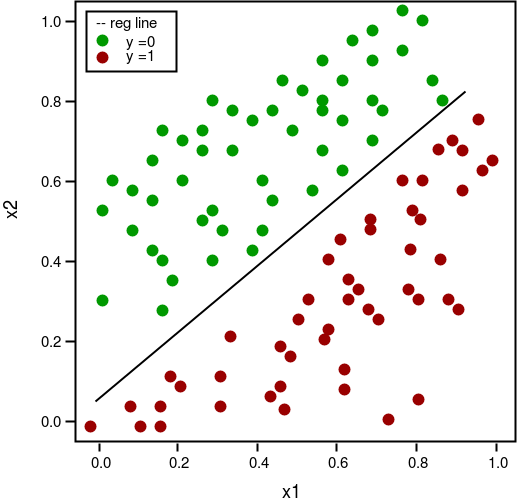
\includegraphics[width=\linewidth]{images/logistic.png}
		\caption{\fontsize{14}{20}\selectfont Demo xác suất logistic}
         (Nguồn:https://benh.edu.vn/logistic-regression-la-gi/)
	\end{center}
\end{figure}
\paragraph{}
Ở hình 3  ta gọi các điểm màu xanh là nhãn 0 và các điểm màu đỏ là nhãn 1 đối với hồi quy logistic ta sẽ biết được với mỗi điểm thì xác xuất rơi vào nhãn 0 là bao nhiêu và xác suất rơi vào nhãn 1 là bao nhiêu, ta có thể thấy giữa hai màu xanh và màu đỏ có một đường thẳng để phân chia rất rõ ràng nhưng nếu các điểm dữ liệu mà không nằm sang hai bên mà nằm trộn lẫn nhiều vào nhau thì ta sẽ phân chia như nào, khi đó ta sẽ gọi tập dữ liệu có nhiều nhiễu và ta phải xử lí trước các nhiễu đó.
\paragraph{}
    Mô hình hồi quy logistic là một mô hình thống kê được sử dụng rộng rãi, chủ yếu được sử dụng cho mục đích phân loại. Có nghĩa là với một tập hợp các quan sát, thuật toán hồi quy Logistic giúp chúng ta phân loại các quan sát này thành hai hoặc nhiều lớp rời rạc. Vì vậy, biến mục tiêu có bản chất rời rạc. Thuật toán hồi quy logistic hoạt động như sau:
\paragraph{}
	Thuật toán hồi quy logistic hoạt động bằng cách thực hiện một phương trình tuyến tính với các biến độc lập hoặc giải thích để dự đoán giá trị phản hồi. 
\paragraph{}
	Phân tích hồi qui logistic là một kỹ thuật thống kê để xem xét mối liên hệ giữa biến độc lập (biến số hoặc biến phân loại) với biến phụ thuộc là biến nhị phân. Trong hồi qui tuyến tính đơn, biến độc lập x và phụ thuộc y là biến số liên tục liên hệ qua phương trình:
\paragraph{}
\begin{figure}[!h]
	\begin{center}
		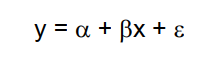
\includegraphics[width=\linewidth]{images/CongThuc1.png}
        \end{center}
\end{figure}
\paragraph{}
Trong hồi qui logistic sử dujgn cho dự báo thời tiết, biến phụ thuộc y chỉ có 2 trạng thái 1 (có mưa) và 0 (không mưa). Muốn đổi ra biến số liên tục người ta tính xác suất của 2 trạng thái này. Nếu gọi p là xác suất để một biến cố xảy ra (có mưa), thì 1-p là xác suất để biến cố không xảy ra (không mưa). Phương trình hồi qui logistic phát biểu:
\paragraph{}
\begin{figure}[!h]
	\begin{center}
		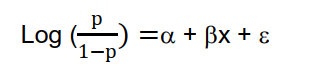
\includegraphics[width=\linewidth]{images/CongThuc3.png}        
	\end{center}
\end{figure}
\paragraph{}
Từ phương trình này, ta có thể tính xác suất dự đoán có mưa theo trị số của x.

\begin{figure}[!h]
	\begin{center}
		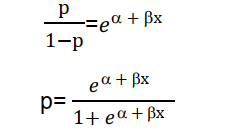
\includegraphics[width=\linewidth]{images/CongThuc2.png}        
	\end{center}
\end{figure}
\pagebreak
\subsubsection{Trong học máy}
\paragraph{}
    Hàm sigmoid được sử dụng để ánh xạ các dự đoán với xác suất. Hàm sigmoid có đường cong hình chữ S. Nó còn được gọi là đường cong sigmoid. Hàm Sigmoid là một trường hợp đặc biệt của hàm Logistic. Nó được đưa ra bởi công thức toán học và được biểu diễn như hình sau:
  \paragraph{}
\begin{figure}[!h]
	\begin{center}
		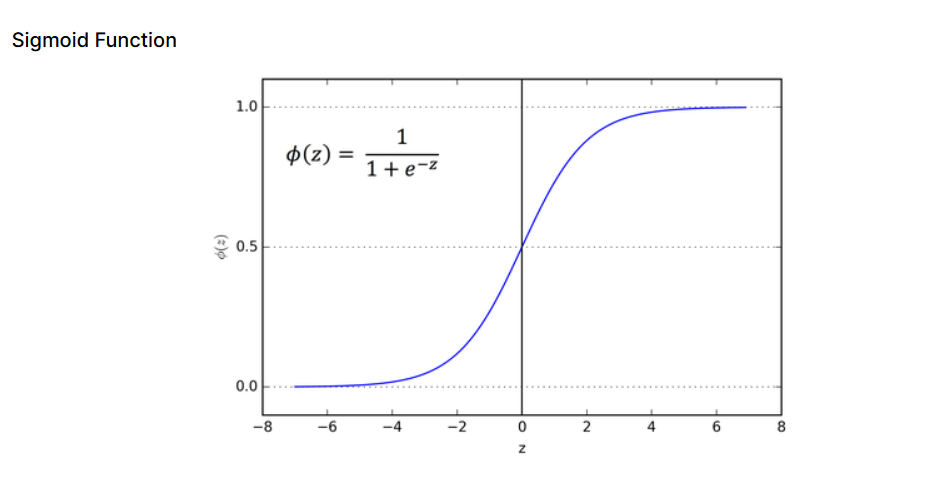
\includegraphics[width=\linewidth]{images/Dothi.png}
		\caption{\fontsize{14}{20}\selectfont Đồ thị Sigmoid Function}
		(Nguồn:https://viblo.asia/p/logistic-regression-bai-toan-co-ban-trong-machine-learning-924lJ4)
	\end{center}
\end{figure}

\paragraph{}
Hàm sigmoid trả về giá trị xác suất từ 0 đến 1. Giá trị xác suất này sau đó được ánh xạ tới một lớp rời rạc là “0” hoặc “1”. Để ánh xạ giá trị xác suất này tới một lớp rời rạc (đạt / không đạt, có / không, đúng / sai).
\subsubsection{Phân loại Logistic Regression}
\paragraph{}
    Mô hình hồi quy logistic có thể được phân loại thành ba nhóm dựa trên các loại biến mục tiêu. Ba nhóm này được mô tả dưới đây: 
\paragraph{}
Hồi quy logistic nhị phân:biến phụ thuộc chỉ có hai 2 kết quả / lớp có thể có.
\paragraph{}
Ví dụ: Nam hoặc Nữ, 0 hoặc 1, ác tính hoặc lành tính, đạt hoặc không đạt, được chấp nhận hoặc không được chấp nhận, có hoặc không, tốt hoặc xấu, đúng hoặc sai, spam hoặc không spam.

\paragraph{}Hồi quy logistic đa thức: xử lý các trường hợp khi  biến phụ thuộc chỉ có hai hoặc 3 kết quả / lớp có thể có trở lên mà không cần sắp xếp thứ tự.
 \paragraph{}
 Ví dụ: Dự đoán chất lượng thực phẩm. (Tốt, Tuyệt vời và Xấu), việc hình ảnh X-quang lồng ngực làm các đặc điểm cho biết về một trong ba kết quả có thể xảy ra (Không có bệnh, Viêm phổi do Vi rút, COVID-19).


\paragraph{}Hồi quy Logistic thứ tự: biến phụ thuộc chỉ có hai hoặc nhiều hơn 3 kết quả / lớp có thể có với thứ tự.
    \paragraph{}
    Ví dụ: Xếp hạng sao từ 1 đến 5, kết quả học tập của học sinh có thể được phân loại là kém, trung bình, tốt và xuất sắc.
  

\subsubsection{Ưu điểm khi sử dụng Logistic Regression}

\paragraph{}Logistic Regression là một trong những thuật toán học máy đơn giản nhất và dễ thực hiện nhưng mang lại hiệu quả lớn cũng như mô hình với thuật toán này không yêu cầu khả năng tính toán cao.

\paragraph{}Các tham số dự đoán đưa ra suy luận về tầm quan trọng của từng tính năng. Hướng liên kết tức là tích cực hoặc tiêu cực cũng được đưa ra.

\paragraph{}Thuật toán này cho phép các mô hình được cập nhật dễ dàng để phản ánh dữ liệu mới. Việc cập nhật có thể được thực hiện bằng cách sử dụng descent gradient ngẫu nhiên.

\paragraph{}Logistic Regression đưa ra các xác suất được hiệu chỉnh tốt cùng với kết quả phân loại.

\paragraph{}Trong một tập dữ liệu chồi quy logistic ít bị sai lệch hơn.

\paragraph{}Hồi quy logistic đôi khi được sử dụng làm mô hình chuẩn để đo lường hiệu suất, vì nó tương đối nhanh chóng và dễ thực hiện.

\paragraph{}Logistic Regression tỏ ra rất hiệu quả khi tập dữ liệu có các tính năng có thể phân tách tuyến tính.
\subsubsection{Nhược điểm khi sử dụng Logistic Regression}
\paragraph{}Các vấn đề phi tuyến tính không thể được giải quyết bằng hồi quy logistic.
\paragraph{}Không thể xử lý các vấn đề phức tạp bằng cách sử dụng hồi quy logistic và không dự đoán được kết quả liên tục.


\subsubsection{Ứng dụng của Logistic Regression}
\paragraph{}Trong dự báo thời tiết, hồi quy logistic không chỉ dự đoán một ngày trong tương lai có mưa hay không, mà còn dự đoán được xác suất xảy ra mưa.
\paragraph{}Trong ngành Giáo dục, hồi quy logistic có thể được sử dụng để dự đoán: Việc một học sinh có được nhận vào một chương trình đại học hay không dựa trên điểm thi và nhiều yếu tố khác. Trong các nền tảng E-learning để xem liệu học sinh có hoàn thành khóa học đúng hạn hay không dựa trên hoạt động trong quá khứ và các số liệu thống kê khác có liên quan đến vấn đề.
\paragraph{} Trong lĩnh vực kinh doanh, hồi quy logistic có các ứng dụng dự đoán liệu giao dịch thẻ tín dụng của người dùng có gian lận hay không.
\paragraph{}Ngành y tế cũng được hưởng lợi từ hồi quy logistic thông qua các cách sử dụng sau:dự đoán một người có mắc bệnh hay không dựa trên các giá trị thu được từ các báo cáo xét nghiệm hoặc các yếu tố khác nói chung.
Một ứng dụng rất sáng tạo của Học máy đang được các nhà nghiên cứu sử dụng là dự đoán một người có COVID-19 hay không bằng cách sử dụng hình ảnh X-quang Ngực.
\paragraph{}Các ứng dụng khác: Hồi quy logistic tìm thấy các ứng dụng của nó trong tất cả các lĩnh vực chính. Ngoài ra, một số ứng dụng thú vị của nó là: Phân loại email - Thư rác hay không phải thư rác. Phân tích cảm xúc - Một người đang buồn hay vui dựa trên một tin nhắn văn bản. Phát hiện và phân loại đối tượng - Phân loại hình ảnh thành hình ảnh mèo hoặc hình ảnh con chó.
\paragraph{}Với dataset, tôi sẽ tạo mô hình hồi quy logistic sử dụng tập dữ liệu Rain in Australia để dự đoán liệu ngày mai trời có mưa hay không, sử dụng hồi quy logistic nhị phân. Mục đích của chúng tôi là tạo ra một mô hình để dự đoán giá trị trong cột RainTomorrow.
\subsection{Giới thiệu về thuật toán Machine Learning rừng ngẫu nhiên (Random Forest Machine Learning)}
\paragraph{}
Random Forest là một Machine Learning được sử dụng để giải quyết các vấn đề hồi quy và phân loại. Nó sử dụng phương pháp học tập hợp, là một kỹ thuật kết hợp nhiều bộ phân loại để đưa ra giải pháp cho các vấn đề phức tạp.
\paragraph{}
Random là ngẫu nhiên, Forest là rừng, nên ở thuật toán Random Forest mình sẽ xây dựng nhiều cây quyết định bằng thuật toán Decision Tree, tuy nhiên mỗi cây quyết định sẽ khác nhau). Sau đó kết quả dự đoán được tổng hợp từ các cây quyết định.
\paragraph{}
Random Forest là một tập hợp của các Decision Tree, mà mỗi cây được chọn theo một thuật toán dựa vào ngẫu nhiên.
\paragraph{}Mỗi cây quyết định đều có những yếu tố ngẫu nhiên: Lấy ngẫu nhiên dữ liệu để xây dựng cây quyết định, lấy ngẫu nhiên các thuộc tính để xây dựng cây quyết định.
\paragraph{}
Decision Tree là tên đại diện cho một nhóm thuật toán phát triển dựa trên Cây quyết định. Ở đó, mỗi Node của cây sẽ là các thuộc tính, và các nhánh là giá trị lựa chọn của thuộc tính đó. Bằng cách đi theo các giá trị thuộc tính trên cây. Cây quyết định sẽ cho ta biết giá trị dự đoán. Nhóm thuật toán cây quyết định có một điểm mạnh đó là có thể sử dụng cho cả bài toán Phân loại (Classification) và Hồi quy (Regression).
\paragraph{}
Giả sử chúng ta muốn đi du lịch tại một địa điểm nào sắp tới, chúng ta sẽ đi hỏi một người bạn để tham khảo ý kiến. Nhưng, ý kiến của người bạn này có thể không khách quan cho lắm. Chúng ta liền đi hỏi thêm một vài người nữa, và tổng hợp lại để cho ra quyết định đi địa điểm đó hay không.
\paragraph{}
Nếu coi mỗi ý kiến của những người góp ý là một cây quyết định, thì chúng ta đã có hình dung được thuật toán Random Forest.
\paragraph{}
Random Forest hoạt động bằng cách đánh giá nhiều cây quyết định ngẫu nhiên, và lấy ra kết quả được đánh giá tốt nhất trong số kết quả trả về.
\subsubsection{Cách thức hoạt động thuật toán Machine Learning rừng ngẫu nhiên}
\paragraph{}Chọn các mẫu ngẫu nhiên từ tập dữ liệu đã cho.
\paragraph{}Thiết lập cây quyết định cho từng mẫu và nhận kết quả dự đoán từ mỗi cây quyết định.
\paragraph{}Hãy bỏ phiếu cho mỗi kết quả dự đoán.
\paragraph{}Chọn kết quả được dự đoán nhiều nhất là dự đoán cuối cùng.
\paragraph{}
\begin{figure}[!h]
	\begin{center}
		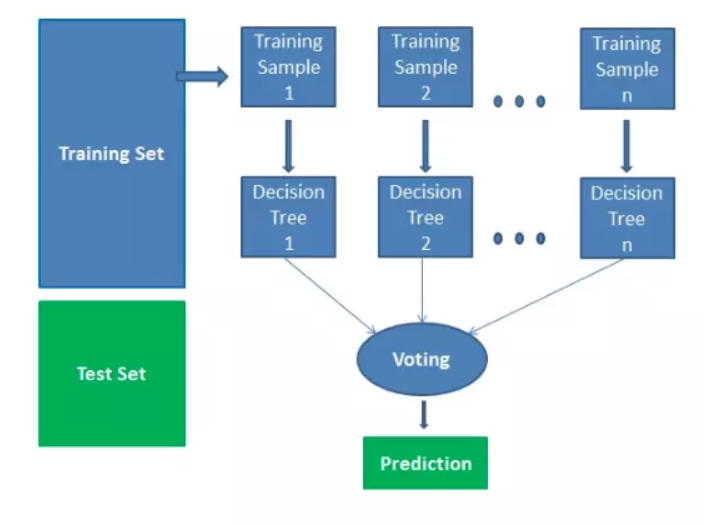
\includegraphics[width=\linewidth]{images/RandomForest.png}
		\caption{\fontsize{14}{20}\selectfont Sơ đồ hoạt động Random Forest}
		(Nguồn:https://viblo.asia/p/phan-lop-bang-random-forests-trong-python-djeZ1D2QKWz)
	\end{center}
\end{figure}
\paragraph{}
\paragraph{}
\paragraph{}
\subsubsection{Ưu điểm thuật toán Machine Learning rừng ngẫu nhiên}
\paragraph{}Áp dụng cho cả bài toán Phân loại (Classification) và Hồi quy (Regression).
\paragraph{}Random forests cũng có thể xử lý các giá trị còn thiếu.
\paragraph{}Xử lý tập dữ liệu lớn với kích thước lớn.
\paragraph{}Có thể tạo mô hình cho các giá trị phân loại.
\paragraph{}Nó không bị vấn đề overfitting.
\subsubsection{Nhược điểm thuật toán Machine Learning rừng ngẫu nhiên}
\paragraph{}Random forests tạo ra dự đoán bởi chậm vì nó có nhiều cây quyết định.
\paragraph{} Random forests tốn thời gian nhiều hơn các thuật toán khác.
\subsubsection{Ứng dụng thuật toán Machine Learning rừng ngẫu nhiên}
\paragraph{}Ngân hàng: Rừng ngẫu nhiên được sử dụng trong ngân hàng để dự đoán mức độ tín nhiệm của người đi vay. Điều này giúp tổ chức cho vay đưa ra quyết định chính xác về việc có cho khách hàng vay hay không. Các ngân hàng cũng sử dụng thuật toán rừng ngẫu nhiên để phát hiện những kẻ gian lận.
\paragraph{}Chăm sóc sức khỏe: Các chuyên gia y tế sử dụng hệ thống rừng ngẫu nhiên để chẩn đoán bệnh nhân. Bệnh nhân được chẩn đoán bằng cách đánh giá tiền sử bệnh trước đây của họ. Hồ sơ y tế trước đây được xem xét để thiết lập liều lượng phù hợp cho bệnh nhân.
\paragraph{}Thị trường chứng khoán: Các nhà phân tích tài chính sử dụng nó để xác định thị trường tiềm năng cho cổ phiếu. Nó cũng cho phép họ xác định hành vi của cổ phiếu.
\paragraph{}Thương mại điện tử: Thông qua các thuật toán rừng mưa, các nhà cung cấp thương mại điện tử có thể dự đoán mức độ yêu thích của khách hàng dựa trên hành vi tiêu dùng trong quá khứ.
\paragraph{}Trong dự báo thời tiết, dự đoán một ngày trong tương lai có mưa hay không, mà còn dự đoán được xác suất xảy ra mưa.
\subsection{Giới thiệu về thuật toán Naive Bayes}
\paragraph{}Naive Bayes Classification (NBC) là một thuật toán dựa trên định lý Bayes về lý thuyết xác suất để đưa ra các phán đoán cũng như phân loại dữ liệu dựa trên các dữ liệu được quan sát và thống kê. Naive Bayes là một trong những thuật toán được ứng dụng rất nhiều trong các lĩnh vực Machine learning dùng để đưa các dự đoán chính xác nhất dự trên một tập dữ liệu đã được thu thập, vì nó khá dễ hiểu và độ chính xác cao.
\subsubsection{Định lý Bayes}
\paragraph{}Định lý Bayes cho phép tính xác suất xảy ra của một sự kiện ngẫu nhiên A khi biết sự kiện liên quan B đã xảy ra. Xác suất này được ký hiệu là P(A|B), và đọc là “xác suất của A nếu có B”. Đại lượng này được gọi xác suất có điều kiện hay xác suất hậu nghiệm vì nó được rút ra từ giá trị được cho của B hoặc phụ thuộc vào giá trị đó.
\paragraph{}Theo định lý Bayes, xác suất xảy ra A khi biết B sẽ phụ thuộc vào 3 yếu tố:
\paragraph{}Xác suất xảy ra A của riêng nó, không quan tâm đến B. Kí hiệu là P(A) và đọc là xác suất của A. Theo nghĩa rằng nó không quan tâm đến bất kỳ thông tin nào về B.
\paragraph{}Xác suất xảy ra B của riêng nó, không quan tâm đến A. Kí hiệu là P(B) và đọc là “xác suất của B”. Đại lượng này còn gọi là hằng số chuẩn hóa (normalising constant), vì nó luôn giống nhau, không phụ thuộc vào sự kiện A.
\paragraph{}Xác suất xảy ra B khi biết A xảy ra. Kí hiệu là P(B|A) và đọc là “xác suất của B nếu có A”. Đại lượng này gọi là khả năng (likelihood) xảy ra B khi biết A đã xảy ra.
\paragraph{}Gọi A, B là hai biến cố
\begin{figure}[!h]
	\begin{center}
		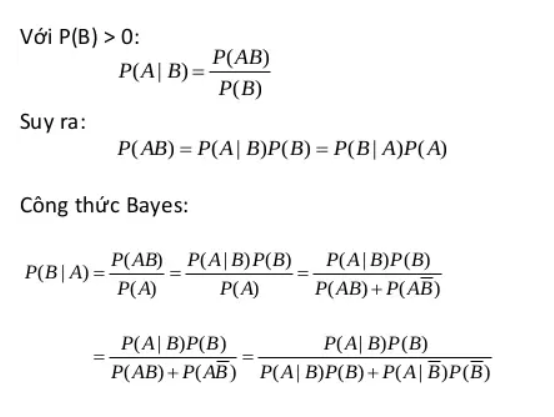
\includegraphics[width=\linewidth]{images/congthucbayes.png}
		\caption{\fontsize{14}{20}\selectfont Công thức Bayes}
		Nguồn: https://viblo.asia/p/thuat-toan-phan-lop-naive-bayes-924lJWPm5PM
	\end{center}
\end{figure}
\paragraph{}Trong đó: P(A|B) là  xác suất xảy ra của một sự kiện ngẫu nhiên A khi biết sự kiện liên quan B đã xảy ra. P(B|A) là xác suất xảy ra B khi biết A xảy ra. P(A) là xác suất sảy ra của riêng A mà không quan tâm đến B. P(B) là xác suất xảy ra của riêng B mà không quan tâm đến A.
\pagebreak{}
\paragraph{}Công thức Bayes tổng quát
\begin{figure}[!h]
	\begin{center}
		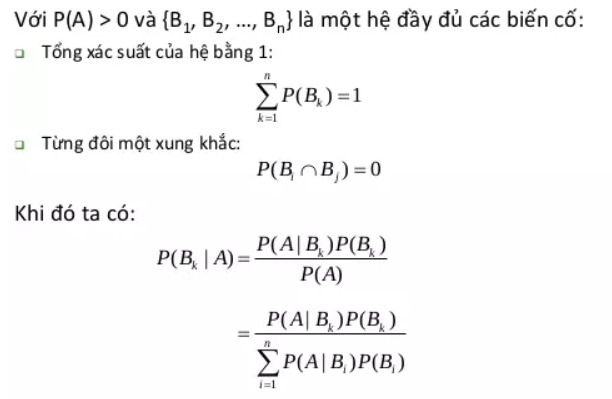
\includegraphics[width=\linewidth]{images/congthuctongquat.png}
		\caption{\fontsize{14}{20}\selectfont Công thức tổng quát}
		Nguồn: https://viblo.asia/p/thuat-toan-phan-lop-naive-bayes-924lJWPm5PM
	\end{center}
\end{figure}
\pagebreak{}
\subsubsection{Các loại phân phối dữ liệu Naive Bayes}
\paragraph{}Phân loại đầu tiên là Gaussian Naive Bayes được sử dụng chủ yếu trong loại dữ liệu mà các thành phần là các biến liên tục. Gaussian (hoặc phân phối chuẩn) là phéptính giá trị trung bình và độ lệch chuẩn từ dữ liệu traiing set. Mô hình Gaussian Naive Bayes từ dữ liệu:
\begin{figure}[!h]
	\begin{center}
		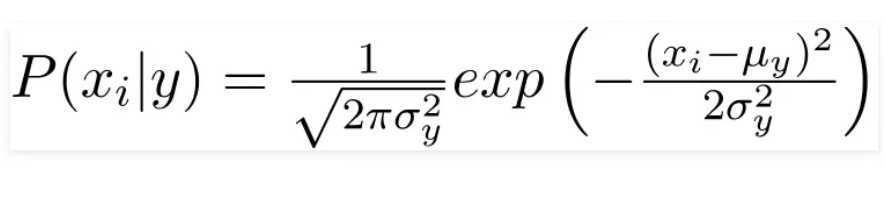
\includegraphics[width=\linewidth]{images/Gaussian.png}
		\caption{\fontsize{14}{20}\selectfont Công thức Gaussian Naive Bayes}
		Nguồn: https://viblo.asia/p/mo-hinh-phan-lop-naive-bayes-vyDZO0A7lwj
	\end{center}
\end{figure}
\paragraph{}Hoặc ta có thể biểu diễn công thức: 
\paragraph{}pdf (x, trung bình, sd) = (1 / (sqrt (2 * PI) * sd)) * exp (- ((x-mean ^ 2) / (2 * sd ^ 2)))
\paragraph{}Trong đó pdf (x) là Gaussian PDF, sqrt () là căn bậc hai, giá trị trung bình và sd là giá trị trung bình và độ lệch chuẩn được tính ở trên, PI là hằng số, exp () là hằng số e hoặc Euler được nâng lên thành công suất và x là giá trị đầu vào cho biến đầu vào.
\paragraph{}Phân loại thức hai là Bernoulli Naive Bayes, mô hình này được áp dụng cho các loại dữ liệu mà mỗi thành phần là một giá trị nhị phân bằng 0 hoặc 1. Ví dụ: cũng với loại văn bản nhưng thay vì đếm tổng số lần xuất hiện của 1 từ trong văn bản, ta chỉ cần quan tâm từ đó có xuất hiện hay không.
\paragraph{}Khi đó p(xi|c) được tính bằng:
\pagebreak{}
\begin{figure}[!h]
	\begin{center}
		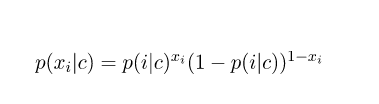
\includegraphics[width=\linewidth]{images/Bernoulli.png}
		\caption{\fontsize{14}{20}\selectfont Công thức Bernoulli Naive Bayes}
		Nguồn: https://www.dataisg.org/tutorial/machine-learning/naive-bayes-classifier
	\end{center}
\end{figure}
\paragraph{}Với p(i|c) là xác xuất từ thứ i xuất hiện trong văn bản của lớp c.
\paragraph{}Phân loại thứ ba là Multinomial Naive Bayes, mô hình này chủ yếu được sử dụng trong phân loại văn bản. Đặc trưng đầu vào ở đây chính là tần suất xuất hiện của từ trong văn bản đó.
\paragraph{}Khi đó, p(xi|c) tỉ lệ với tần suất từ thứ i xuất hiện trong văn bản của class c. Giá trị này được tính bằng:
\begin{figure}[!h]
	\begin{center}
		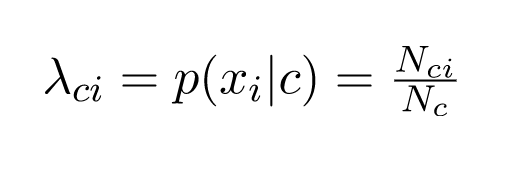
\includegraphics[width=\linewidth]{images/Multinomial.png}
		\caption{\fontsize{14}{20}\selectfont Công thức Multinomial Naive Bayes}
		Nguồn: https://www.dataisg.org/tutorial/machine-learning/naive-bayes-classifier
	\end{center}
\end{figure}
\pagebreak{}
\paragraph{}Với: N(ci) là số lần từ thứ i xuất hiện trong văn bản của lớp c. Được tính bằng tổng của tất cả các thành phần thứ i của vectơ đặc trưng ứng với lớp c. Nc  là tổng số từ xuất hiện trong lớp c, bằng tổng độ dài của toàn bộ văn bản thuộc lớp c.
\subsubsection{Ưu điểm}
\paragraph{}Dễ sử dụng và nhanh khi cần dự đoán nhãn của dữ liệu test. Thực hiện khá tốt trong multiclass prediction.
\paragraph{}
Có thể hoạt động với các vectơ đặc trưng mà một phần là liên tục (sử dụng Gaussian Naive Bayes ), phần còn lại ở dạng rời rạc (sử dụng Multinomial hoặc Bernoulli ).
\paragraph{}
Khi giả định rằng các đặc trưng của dữ liệu là độc lập với nhau thì Naive Bayes chạy tốt hơn các thuật toán khác như logistic regression khi có ít dữ liệu đào tạo.
\paragraph{}Trực quan khi bạn hiểu khái niệm
\paragraph{}Rất dễ triển khai và hoạt động tốt trong dự đoán đa kính
\paragraph{}Nó hoạt động tốt với các biến đầu vào phân loại
\subsubsection{Nhược điểm}
\paragraph{}Độ chính xác của Naive Bayes nếu so với các thuật toán khác thì không được cao.
\paragraph{}
Bất khả thi khi các đặc trưng của dữ liệu là độc lập với nhau.
\subsubsection{Ứng dụng}
\paragraph{}
Dự đoán theo thời gian thực: Vì Naive Bayes nhanh và dựa trên số liệu thống kê của Bayes nên nó hoạt động tốt trong việc đưa ra dự đoán trong thời gian thực. Trên thực tế, rất nhiều mô hình thời gian thực hoặc mô hình trực tuyến phổ biến dựa trên số liệu thống kê của Bayes.
\paragraph{}Dự đoán đa kính (Multiclass prediction): Như đã nói trước đây, Naive Bayes hoạt động tốt khi có nhiều hơn hai lớp cho biến đầu ra.
\paragraph{}Phân loại văn bản (Text classification/ Spam Filtering/ Sentiment Analysis): Phân loại văn bản cũng bao gồm các ứng dụng phụ như lọc thư rác và phân tích tình cảm. Vì Naive Bayes hoạt động tốt nhất với các biến rời rạc, nó có xu hướng hoạt động tốt trong các ứng dụng này.
\paragraph{}Hệ thống đề xuất (Recommendation System): Naive Bayes thường được sử dụng cùng với các thuật toán khác như lọc cộng tác để xây dựng các hệ thống đề xuất như phần đề xuất của Netflix hoặc các sản phẩm được đề xuất của Amazon hoặc các bài hát được đề xuất của Spotify.
\paragraph{}Với dataset, tôi sẽ tạo mô hình Bernoulli Naive Bayes và Gaussian Naive Bayes sử dụng tập dữ liệu Rain in Australia để dự đoán liệu ngày mai trời có mưa hay không. Mục đích của chúng tôi là tạo ra một mô hình để dự đoán giá trị trong cột RainTomorrow.
\pagebreak
\subsection{Giới thiệu về thuật toán XGBoost}
\paragraph{}Trong các vấn đề dự đoán liên quan đến dữ liệu phi cấu trúc (hình ảnh, văn bản, v.v.), mạng neural có xu hướng vượt trội hơn tất cả các thuật toán hoặc framework khác. Tuy nhiên, khi nói đến dữ liệu dạng bảng / dữ liệu có cấu trúc các thuật toán tree-based xử lý rất tốt. 
\paragraph{}
Thuật toán XGBoost thuộc nhóm các thuật toán tree-based được phát triển như một dự án nghiên cứu tại Đại học Washington và là phiên bản cải tiến của Gradient Boosting.
\paragraph{}XGBoost có thể được sử dụng để giải quyết được tất cả các vấn đề từ hồi quy (regression), phân loại (classification), ranking và giải quyết các vấn đề do người dùng tự định nghĩa.
\paragraph{}Tốc độ xử lý: XGBoost thực hiện tinh toán song song nên tốc độ xử lý có thể tăng gấp 10 lần so với GBM. Ngoài ra, XGboost còn hỗ trợ tính toán trên Hadoop.
\paragraph{}Overfitting: XGBoost áp dụng cơ chế Regularization nên hạn chế đáng kể hiệ tượng Overfitting (GBM không có regularization).
\paragraph{}Sự linh hoạt: XGboost cho phép người dùng sử dụng hàm tối ưu và chỉ tiêu đánh giá của riêng họ, không hạn chế ở những hàm cung cấp sẵn.
\paragraph{}Xử lý missing value: XGBoost bao gồm cơ chế tự động xử lý missing value bên trong nó. Vì thế, có thể bỏ qua bước này khi chuẩn bị dữ liệu cho XGBoost.
\paragraph{}Tự động cắt tỉa: Tính năng tree pruning hộ trợ việc tự động bỏ qua những leaves, nodes không mang giá trị tích cực trong quá trình mở rộng tree.
\paragraph{}Với dataset, tôi sẽ tạo mô hình XGBoost sử dụng tập dữ liệu Rain in Australia để dự đoán liệu ngày mai trời có mưa hay không. Loading dữ liệu, phân tách dữ liệu xử lý missing value và tạo train test. Mục đích của chúng tôi là tạo ra một mô hình để dự đoán giá trị trong cột RainTomorrow.
\pagebreak
\section*{CHƯƠNG 3 - DỮ LIỆU THỰC NGHIỆM}
\addcontentsline{toc}{section}{CHƯƠNG 3 - DỮ LIỆU THỰC NGHIỆM}
\setcounter{section}{3}
\setcounter{subsection}{0}
\subsection{Đặc tả dữ liệu thực nghiệm}
\paragraph{}
	Dữ liệu có liên quan trực tiếp đến dự báo thời tiết của một quốc gia. Dữ liệu weatherAUS.csv được nghiên cứu bao gồm: Nhiệt độ, lượng mưa, độ bốc hơi, độ ẩm, áp xuất, hướng gió, vận tốc gió và mật độ mây được thu thập trong 10 năm (từ 1/12/2008 đến 25/6/2017) ở 49 trạm khí tượng của nước Úc.
    \begin{figure}[!h]
	\begin{center}
		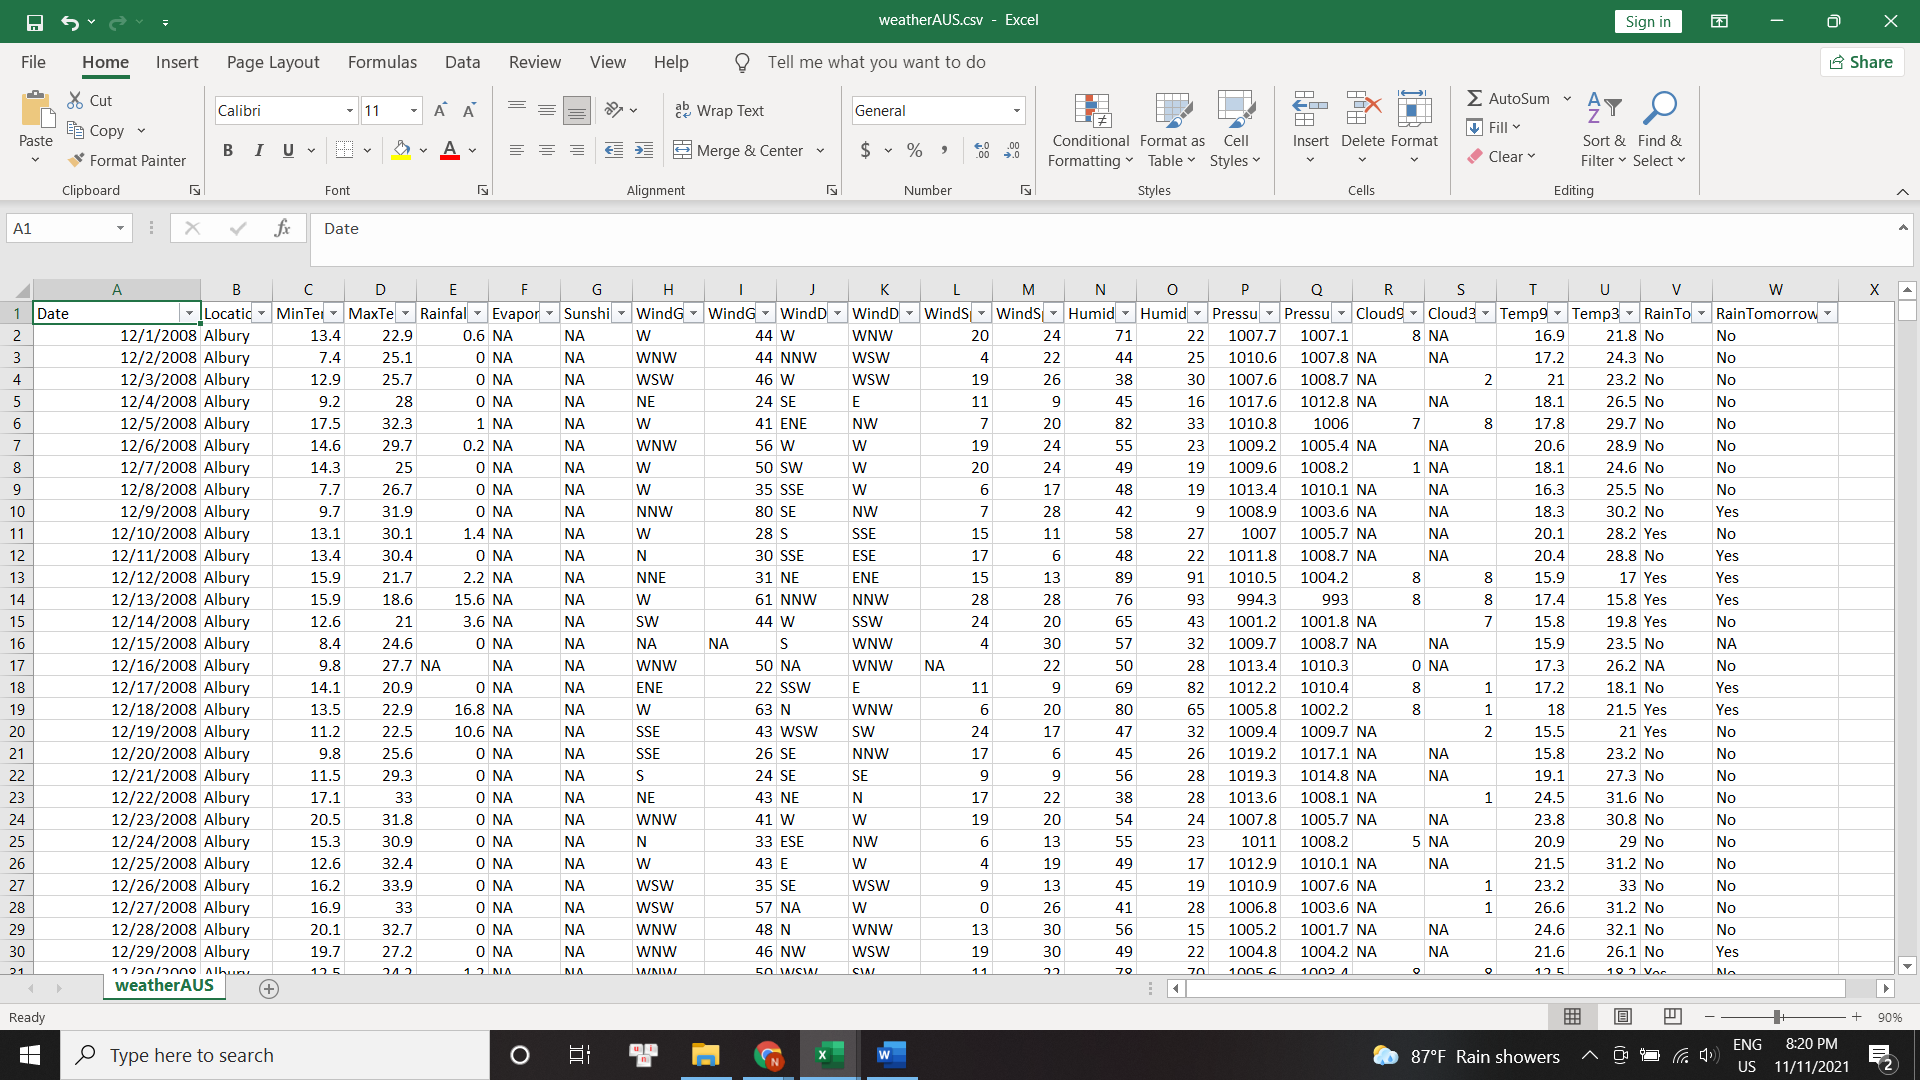
\includegraphics[width=\linewidth]{images/dataset.png}
		\caption{\fontsize{14}{20}\selectfont Dataset thời tiết ở Úc}      
	\end{center}
\end{figure}
\paragraph{}
    Link dataset: https://www.kaggle.com/jsphyg/weather-dataset-rattle-package
\paragraph{} Dữ liệu thực tế được ghi nhận tại Australia trong 10 năm liền có 145460 dòng với 23 thuộc tính bao gồm 2 thuộc tính RainToday, RainTomorrow.
\paragraph{} Date: ngày tháng năm thu thập dòng dữ liệu (mm/dd/yyyy).
\paragraph{} Location: địa điểm (name).
\paragraph{} MinTemp: nhiệt độ tối thiểu (oC).
\paragraph{} MaxTemp: nhiệt độ tối đa (oC).
\paragraph{} Rainfall: lượng mưa được ghi nhận trong ngày (mm).
\paragraph{} Evaporation: sự bốc hơi được ghi nhận từ 24 giờ đêm đến 9h sáng (mm).
\paragraph{} Sunshine: số giờ nắng trong ngày (hour).
\paragraph{} WindGustDir: hướng gió (N-E-W-S).
\paragraph{} WindGustSpeed: vận tốc gió (km/h).
\paragraph{} WindDir9am: hướng gió lúc 9 giờ sáng (N-E-W-S).
\paragraph{} WindDir3pm: hướng gió lúc 3 giờ chiều (N-E-W-S).
\paragraph{} WindSpeed9am: vận tốc gió lúc 9 giờ sáng (km/h).
\paragraph{} WindSpeed3pm: vận tốc gió lúc 3 giờ chiều (km/h).
\paragraph{} Humidity9am: độ ẩm không khí lúc 9 giờ sáng (g/m3).
\paragraph{} Humidity3pm: độ ẩm không khí lúc 3 giờ chiều (g/m3).
\paragraph{} Pressure9am: áp suất không khí lúc 9 giờ sáng (N/m2).
\paragraph{} Pressure3pm: áp suất không khí lúc 3 giờ chiều (N/m2).
\paragraph{} Cloud9am: mật độ mây theo các mức độ lúc 9 giờ sáng (0-9).
\paragraph{} Cloud3pm: mật độ mây theo các mức độ lúc 3 giờ chiều (0-9).
\paragraph{} Temp9am: nhiệt độ ghi nhận lúc 9 giờ sáng (oC).
\paragraph{} Temp3pm: nhiệt độ ghi nhận lúc 3 giờ chiều (oC).
\paragraph{} RainToday: thuộc tính ghi nhận mưa trong ngày (yes/no).
\paragraph{} RainTomorrow: thuộc tính dự đoán mưa trong ngày tiếp theo (yes/no).
\paragraph{} Với các dữ liệu bị thiếu trong dataset weatherAUS.csv sẽ được xử lý missing value như sau:
\paragraph{}Bước 1: Loading dataset
\paragraph{}Bước 2: Phân tích các thuộc tính thành 2 loại (kiểu số và kiểu kí tự).
\paragraph{}Bước 3: Có nhiều cách xử lý dữ liệu bị thiếu: Sử dụng trung vị hoặc giá trị trung bình, chọn giá trị ngẫu nhiên để đưa vào hoặc giá trị có tần suất xuất hiện nhiều nhất của mỗi thuộc tính
\paragraph{}Ở trường hợp dataset này sử dụng điền các giá trị còn thiếu bằng giá trị có tần suất xuất hiện nhiều nhất của mỗi thuộc tính
\paragraph{}Sử dụng hàm fillna() để tìm dữ liệu xuất hiện nhiều nhất lấp vào chỗ trống.
\subsection{Thực nghiệm bằng đồ thị dùng phần mềm Tableau}
\begin{figure}[!h]
	\begin{center}
		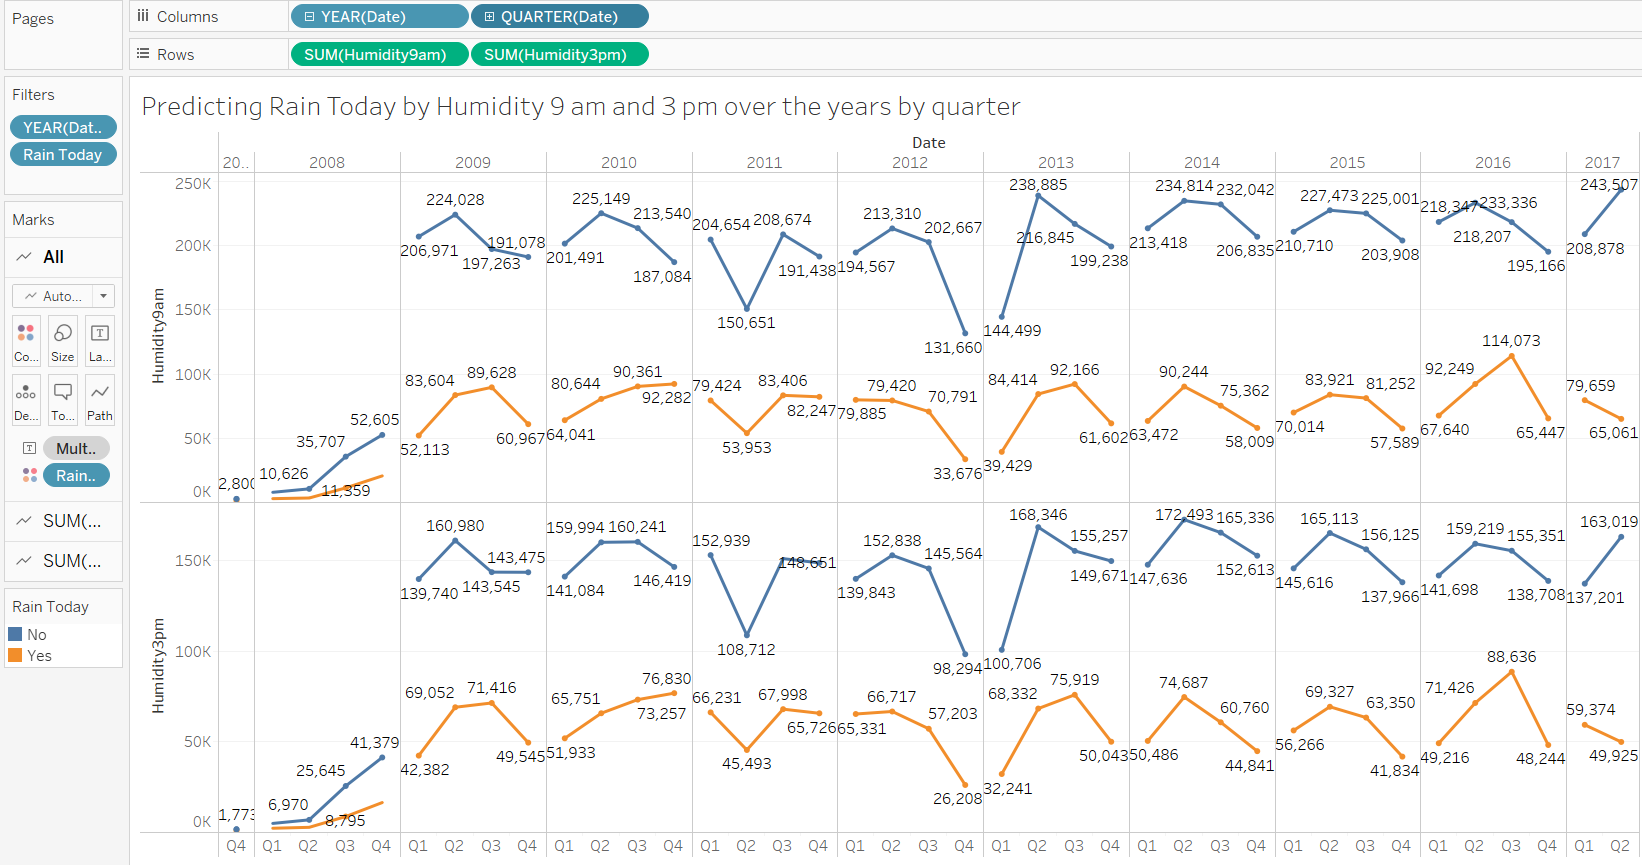
\includegraphics[width=\linewidth]{images/tableau1.png}
		\caption{\fontsize{14}{20}\selectfont Biểu đồ dự đoán hôm nay trời mưa qua độ ẩm 9h sáng và 3h chiều theo từng quý (2007-2017)}
	\end{center}
\end{figure}
\paragraph{}\paragraph{}\paragraph{}\paragraph{}
\paragraph{}Biểu diễn được sự khác biệt giữa độ ẩm lúc 9 giờ sáng và 3 giờ chiều cho thấy được tổng độ ẩm vào lúc 3 giờ ở nước Úc thường thấp hơn lúc 9 giờ sáng thấp nhất là 1773 g/m3 thấp hơn là 2800 g/m3 độ ẩm thấp nhất vào lúc 9 giờ sáng được ghi số liệu vào năm 2007 quý 4. Và tổng độ ẩm cao nhất 9 giờ sáng là 243507 g/m3 vào quý 2 năm 2017 với buổi chiều độ ẩm cao nhất được ghi nhận là vào quý 2 năm 2014 là 1724936 g/m3. Kết luận dù cho độ ẩm cao nhưng cũng không trời mưa thông qua dự đoán giá trị No, phân tích cho thấy độ ẩm No cao hơn phần giá trị Yes, cho nên hôm nay có mưa không phụ thuộc vào độ ẩm cao.
\pagebreak{}
\begin{figure}[!h]
	\begin{center}
		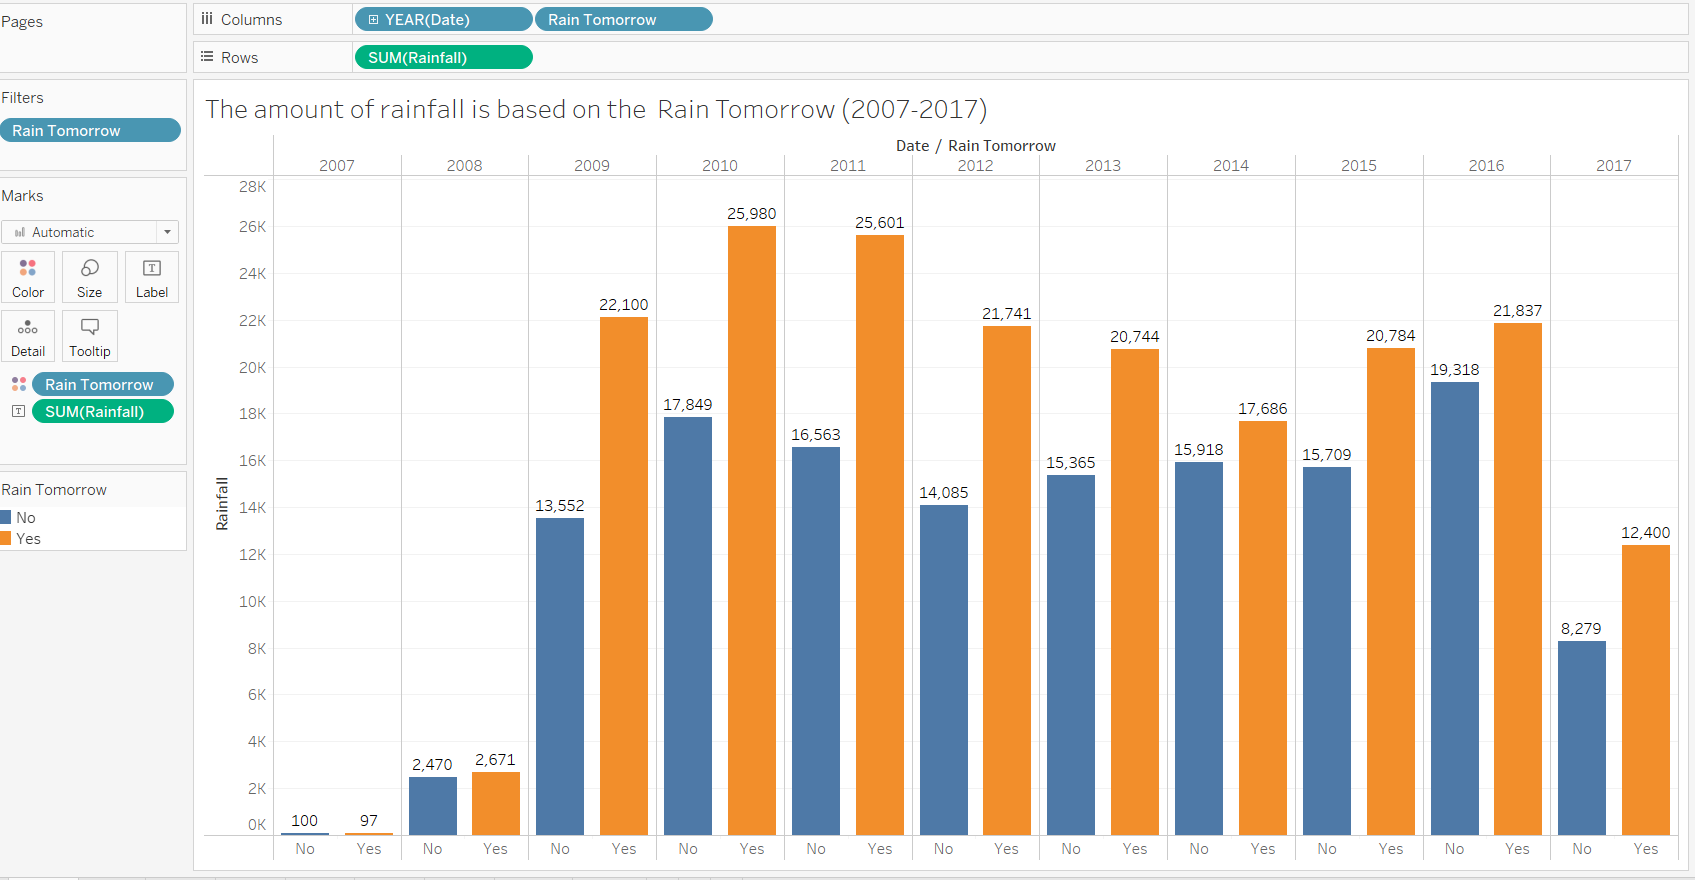
\includegraphics[width=\linewidth]{images/tableau2.png}
		\caption{\fontsize{14}{20}\selectfont Biểu đồ cột thể hiện số tổng lượng mưa sẽ rơi qua dự đoán ngày mai có mưa hay không (2007-2017).}
	\end{center}
\end{figure}
\paragraph{}Tổng lượng mưa sẽ rơi thể hiện qua giá trị Yes từ năm 2008 cao hơn hẳn tổng lượng mưa sẽ không rơi qua giá trị No. Minh chứng từ năm 2008 giá trị Yes là 2671 mm cao hơn với 2470 mm giá trị No. Và tổng lượng mưa rơi cao nhất của Yes là 25980mm so với lượng mưa No trong năm đó chỉ 17 849 mm khẳng định năm đó sẽ trời đổ mưa nhiều hơn so các năm còn lại. Kết luận có thể năm 2007 có lượng mưa giá trị Yes thấp hơn lượng mưa so với gái trị No thì năm đó RainTomorrow có dự báo thời tiết trời đổ mưa ít hơn so với các năm khác.
\pagebreak{}
\begin{figure}[!h]
	\begin{center}
		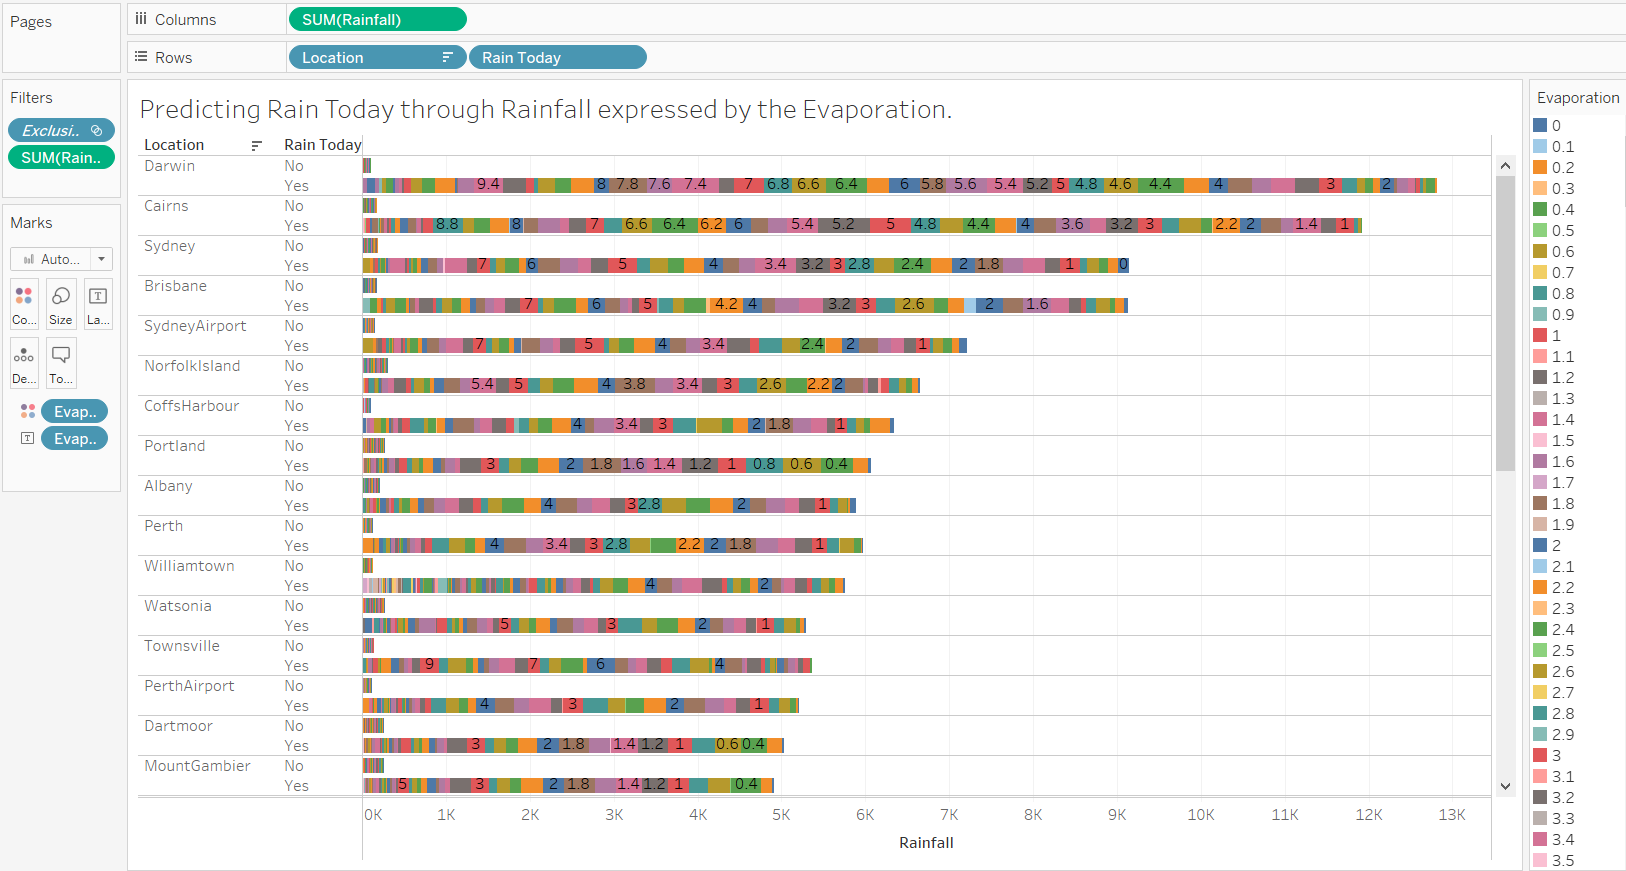
\includegraphics[width=\linewidth]{images/tableau3.png}
		\caption{\fontsize{14}{20}\selectfont Biểu đồ cột ngang thể hiện dự đoán hôm nay trời sẽ mưa qua tổng lượng mưa sẽ rơi thể hiện theo thuộc tính Evaporation(sự bốc hơi)}
	\end{center}
\end{figure}
\paragraph{}Biểu đồ cho biết sự bốc hơi ở khắp nước Úc kèm theo lượng mưa được ghi nhận trong ngày có qua dự đoán hôm nay có mưa hay không(Yes/No), có bỏ qua một vài địa điểm có giá trị null về sự bốc hơi, nơi được ghi nhận số liệu sự bốc hơi của nước Úc tốt nhất là Darwin có chỉ số cụ thể rõ ra và lượng mưa trong ngày ghi nhận cũng cao nhất gần 13000mm và với độ bốc hơi được thể hiện liên tục từ 0 cho đến 8.8 mm. Kết luận rằng ngày có lượng mưa thấp cũng lại có giá trị dự đoán No, trời sẽ không mưa, hiển nhiên có lượng mưa cao và thể hiện được độ bốc hơi cao thì có khả năng trời sẽ mưa thể hiện qua giá trị Yes.
\pagebreak{}
\begin{figure}[!h]
	\begin{center}
		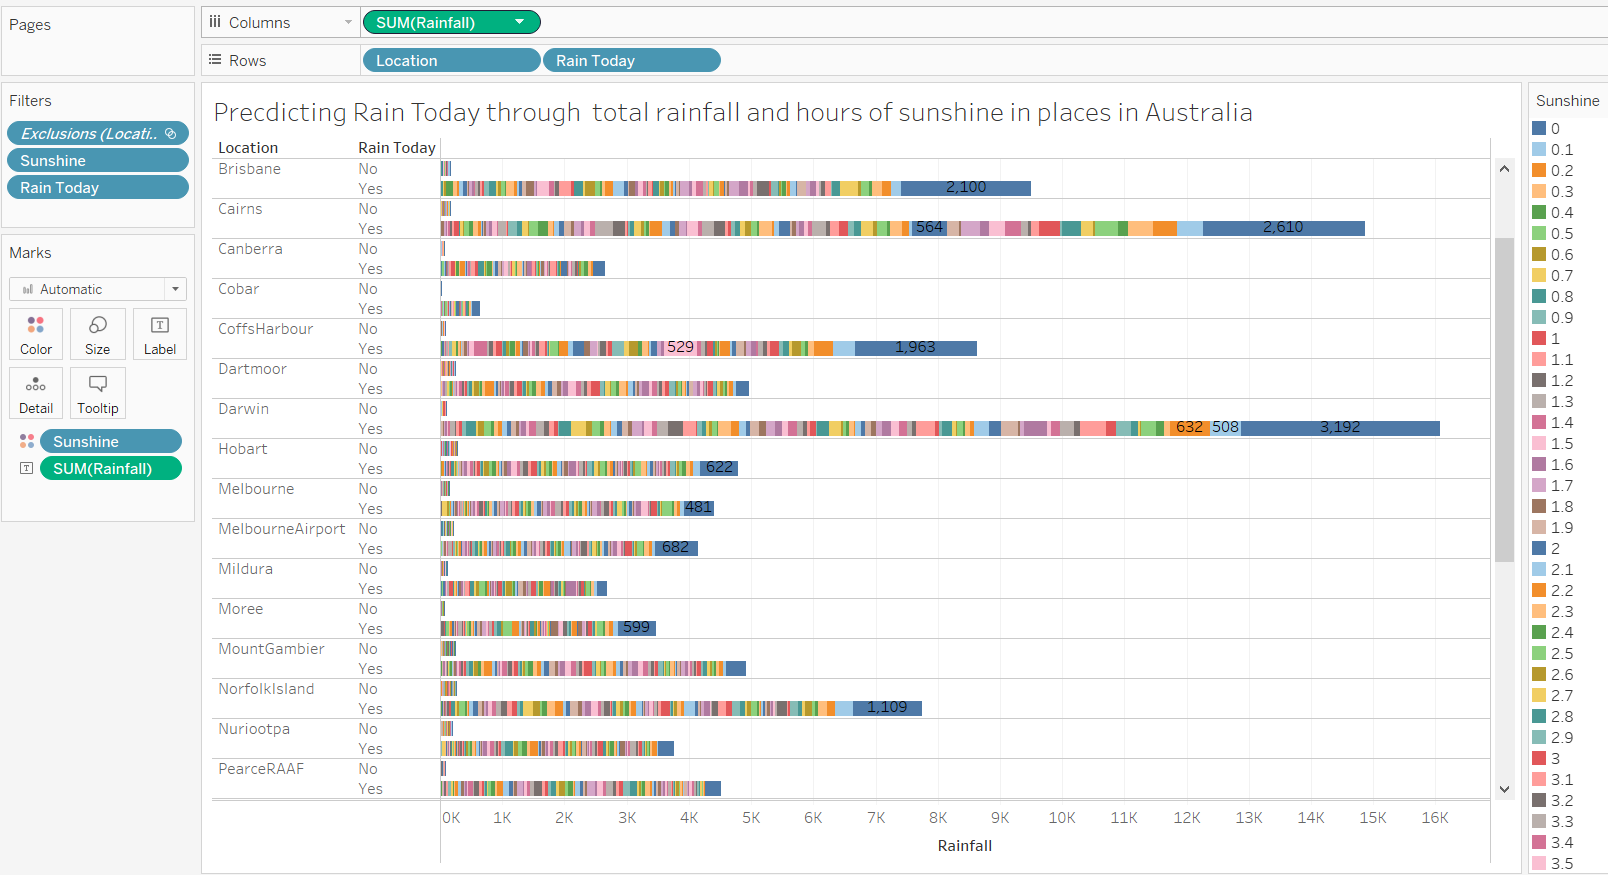
\includegraphics[width=\linewidth]{images/tableau4.png}
		\caption{\fontsize{14}{20}\selectfont Biểu đồ cột ngang thể hiện số giờ nắng được ghi nhận trong ngày kèm theo tổng lượng mưa sẽ rơi ở khắp nơi nước Úc.}
	\end{center}
\end{figure}
\paragraph{}Cho ta thấy rằng Darwin là nơi ghi nhận tốt nhất về tổng lượng mưa cao nhất như khoảng 3192 mm, số giờ nắng ghi nhận được trong ngày dựa vào bảng màu bên phải thì tương ứng là 0 giờ. Và có xóa đi những nơi không ghi nhận được số giờ nắng có giá trị null, và nơi có tổng lượng mưa được ghi nhận trong ngày thấp là Cobar được ghi nhận với lượng mưa chưa tới 1000 mm thì có lẽ số ngày nắng ghi nhận được có khi lại cao hơn. Do nếu ghi nhận được số giờ nắng cao thì tổng lượng mưa hôm đó rới sẽ rất thấp vì chúng nó trái nghịch nhau.
\pagebreak{}
\begin{figure}[!h]
	\begin{center}
		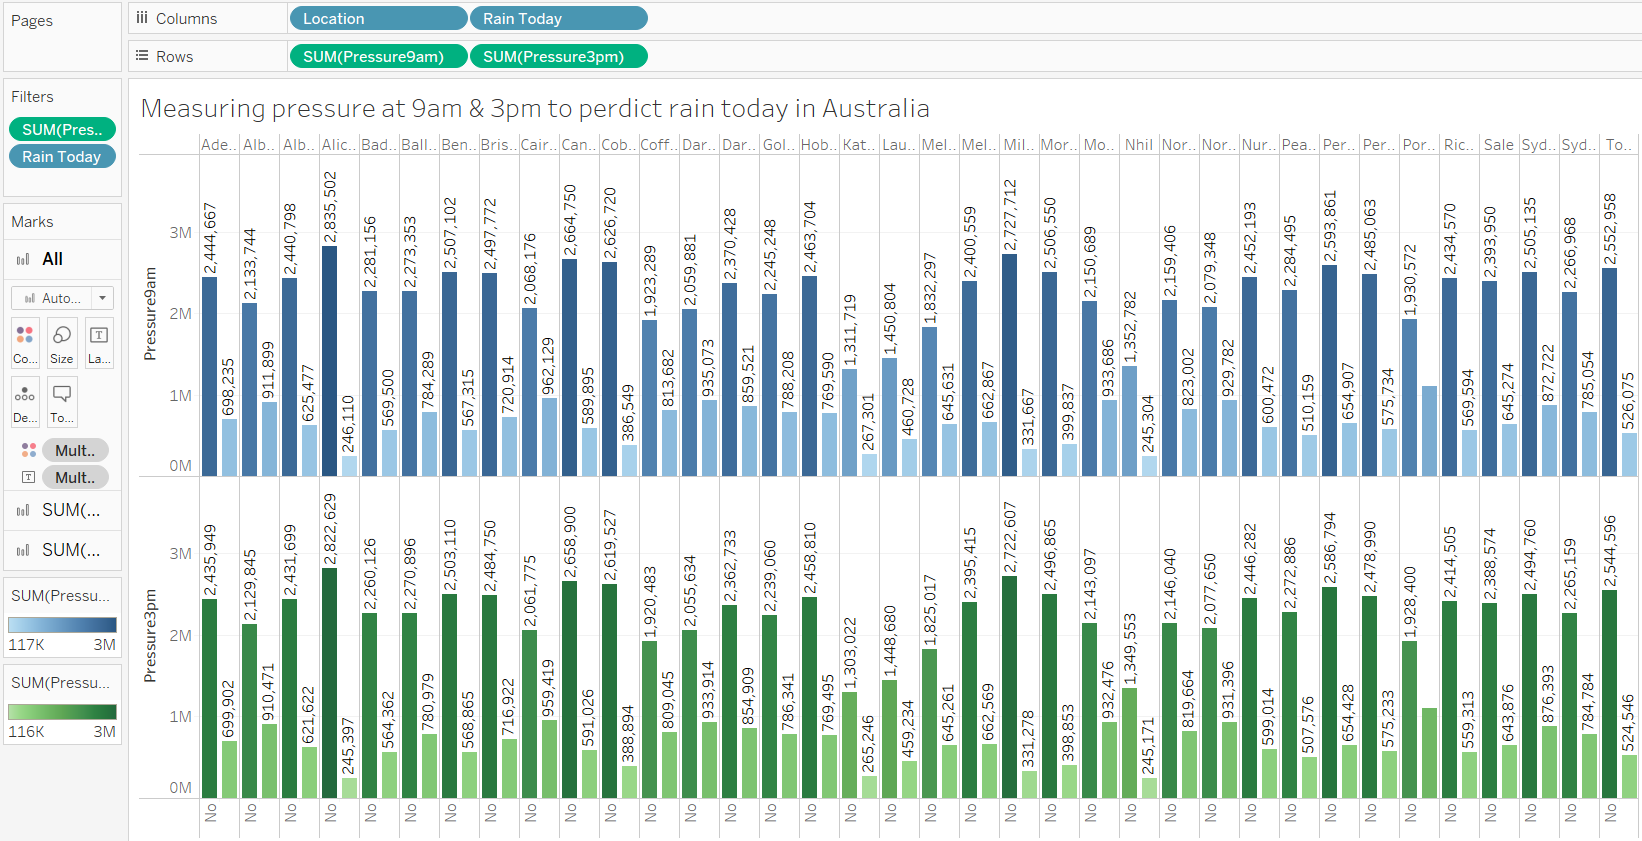
\includegraphics[width=\linewidth]{images/tableau5.png}
		\caption{\fontsize{14}{20}\selectfont Biểu đồ cột hiển thị tổng áp suất không khí đo được lúc 9 giờ sáng và 3 giờ chiều ở nước Úc}
	\end{center}
\end{figure}
\paragraph{}Tổng áp suất không khí lúc 9 giờ sáng luôn lớn hơn tổng áp suất không khí lúc 3 giờ chiều. Và áp suất không khí cao thì ghi nhận mưa trong ngày là giá trị No, vậy nghĩa là ấp suất không khí thấp thì hôm đó ghi nhận được trời sẽ đổ mưa trong ngày.
\pagebreak{}
\begin{figure}[!h]
	\begin{center}
		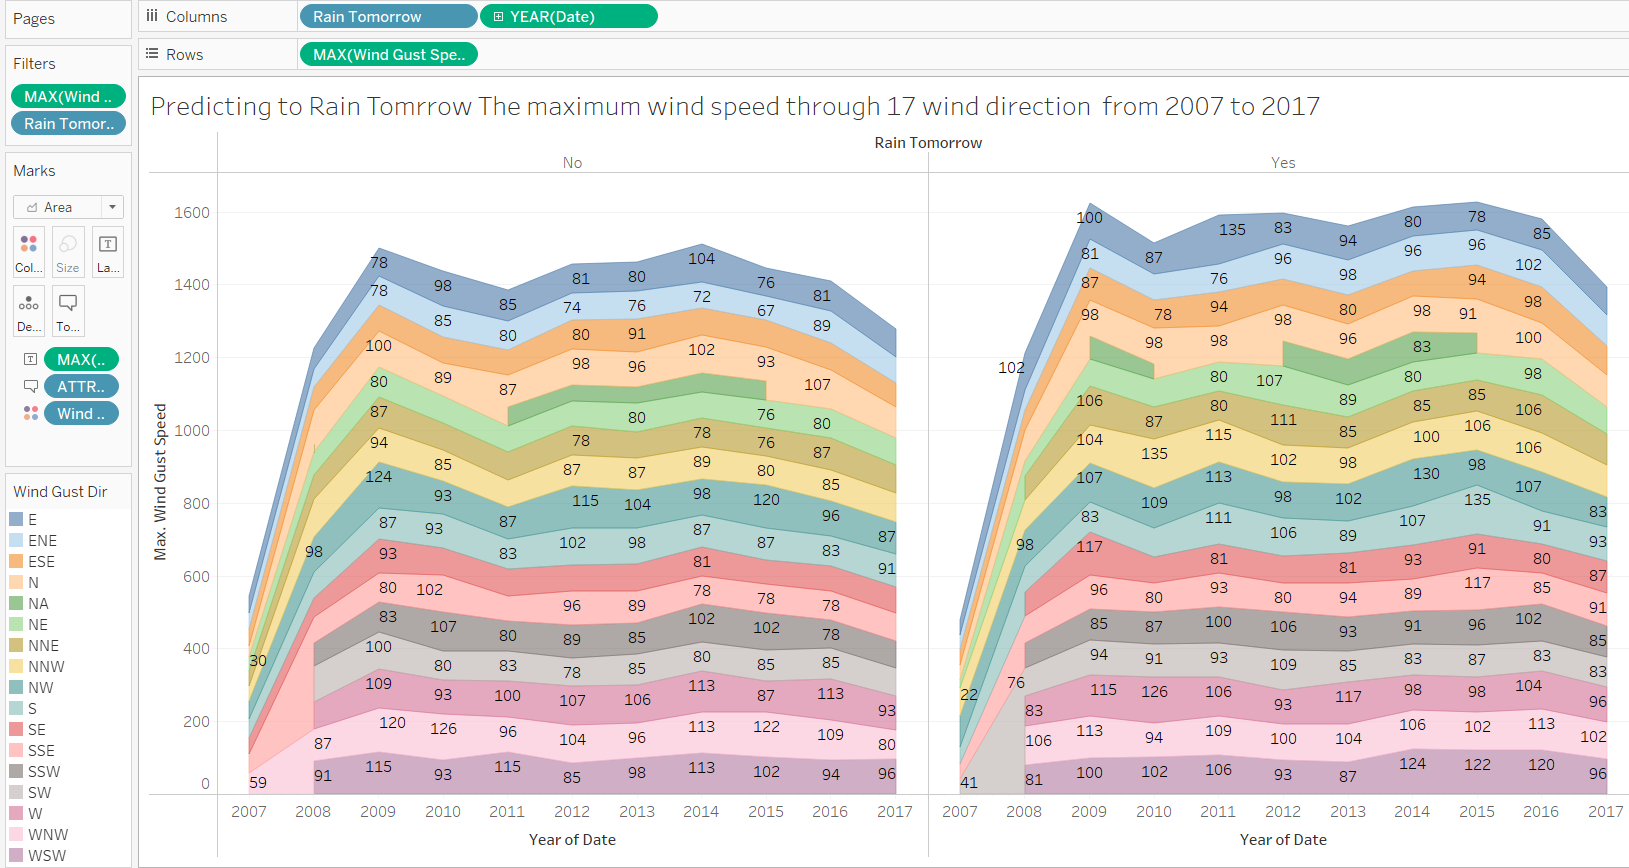
\includegraphics[width=\linewidth]{images/tableau6.png}
		\caption{\fontsize{14}{20}\selectfont Biểu đồ rời rạc dự đoán mưa vào ngày tiếp theo với vận tốc gió lúc 24 giờ lớn nhất qua các hướng gió (2007 – 2017)}
	\end{center}
\end{figure}
\paragraph{}Vận tốc gió lớn nhất lên tới 135 km/h hay thổi qua hướng NNW là hướng Bắc Tây Bắc và S là hướng phía Nam cụ thể tuần tự từng đợt là vào năm 2010 và năm 2015 qua giá trị Yes. Qua đó ta thấy được dự đoán mai sẽ mưa thì vận tốc gió lúc 24 giờ cũng lớn hơn.
\pagebreak{}
\begin{figure}[!h]
	\begin{center}
		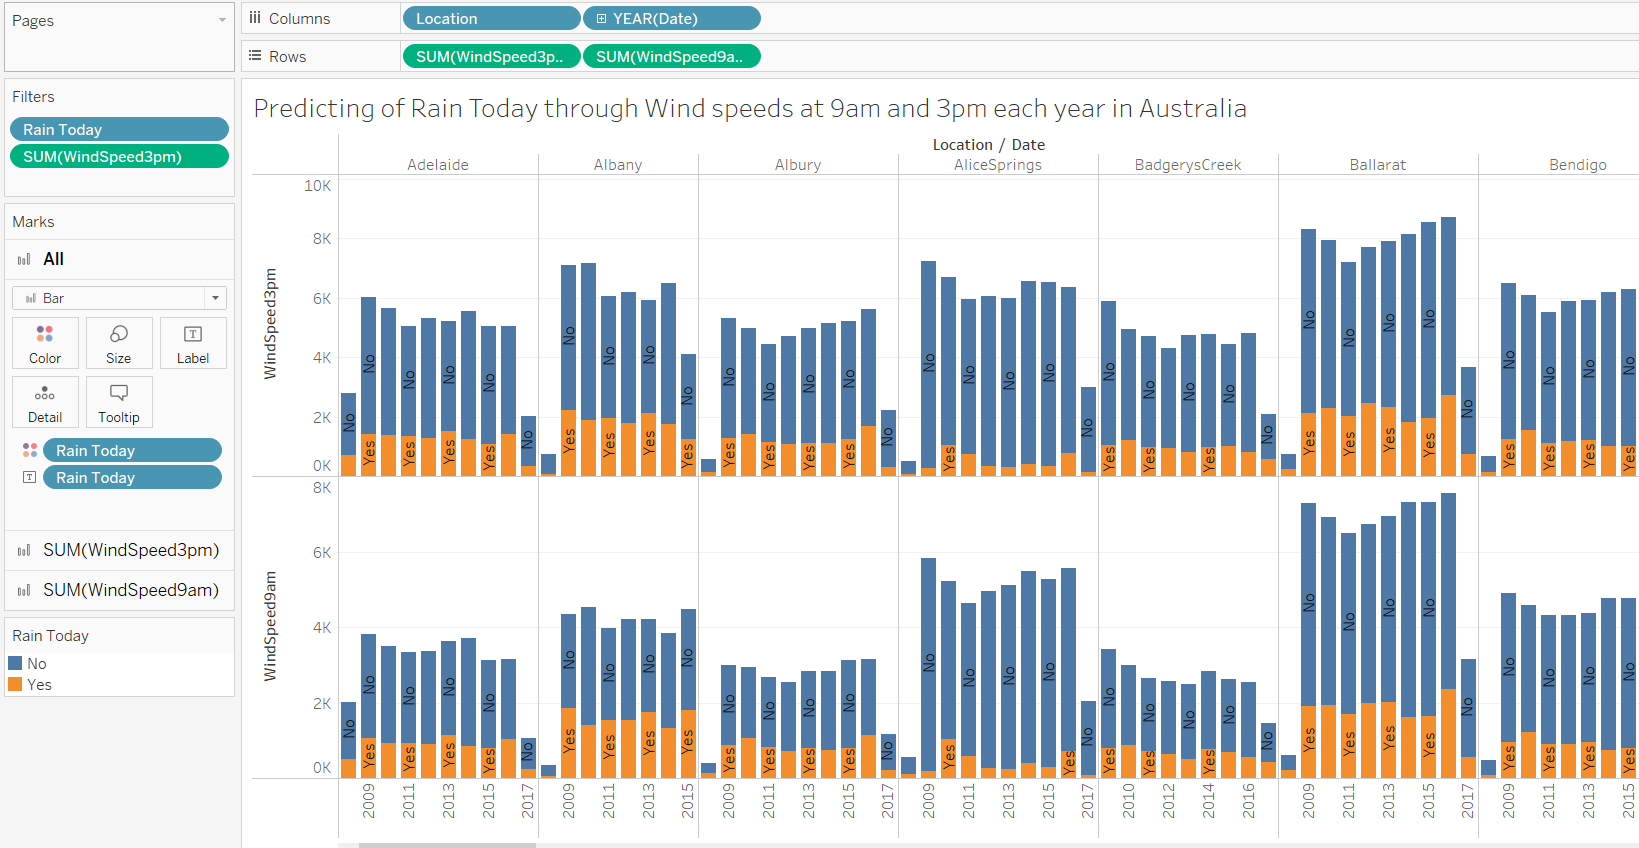
\includegraphics[width=\linewidth]{images/tableau7.png}
		\caption{\fontsize{14}{20}\selectfont Biểu đồ cột ghi nhận mưa trong ngày qua tốc độ gió lúc 9 giờ sáng và 3 giờ chiều qua mỗi năm ở nước Úc}
	\end{center}
\end{figure}
\pagebreak{}
\begin{figure}[!h]
	\begin{center}
		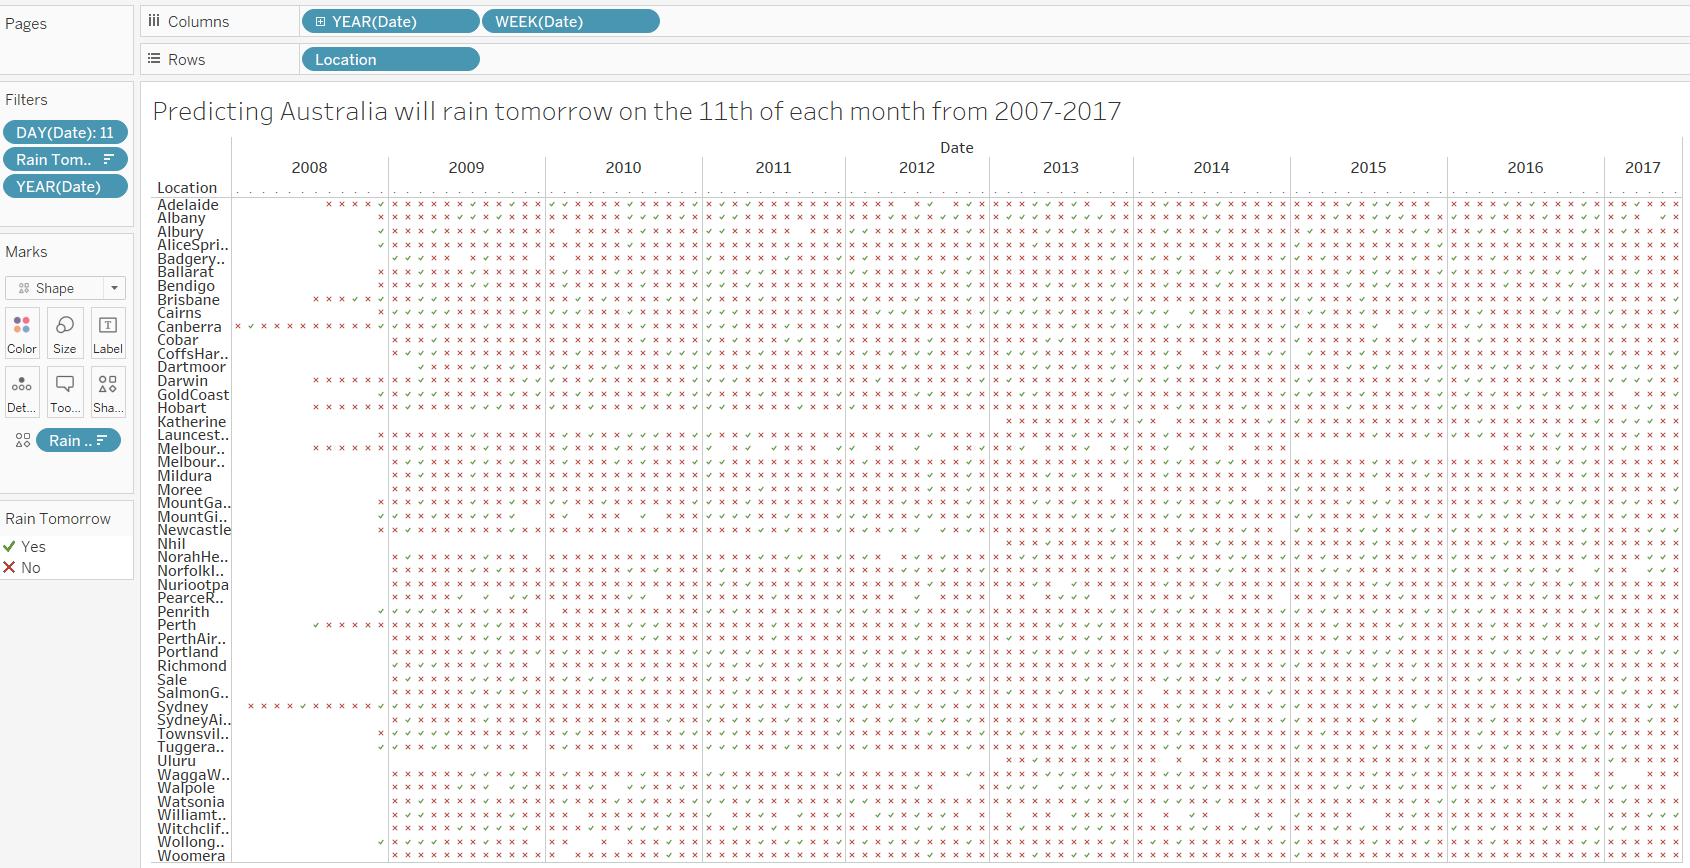
\includegraphics[width=\linewidth]{images/tableau8.png}
		\caption{\fontsize{14}{20}\selectfont Biểu đồ bảng dự đoán mai những nơi ở nước Úc sẽ có mưa vào ngày 11 mỗi tháng từ năm 2007-2017}
	\end{center}
\end{figure}
\paragraph{}Qua đó ta thấy được nước Úc rất ít những ngày dự đoán mai có mưa chỉ chọn qua một ngày cụ thể của mỗi tháng trải qua 10 năm.
\pagebreak{}
\begin{figure}[!h]
	\begin{center}
		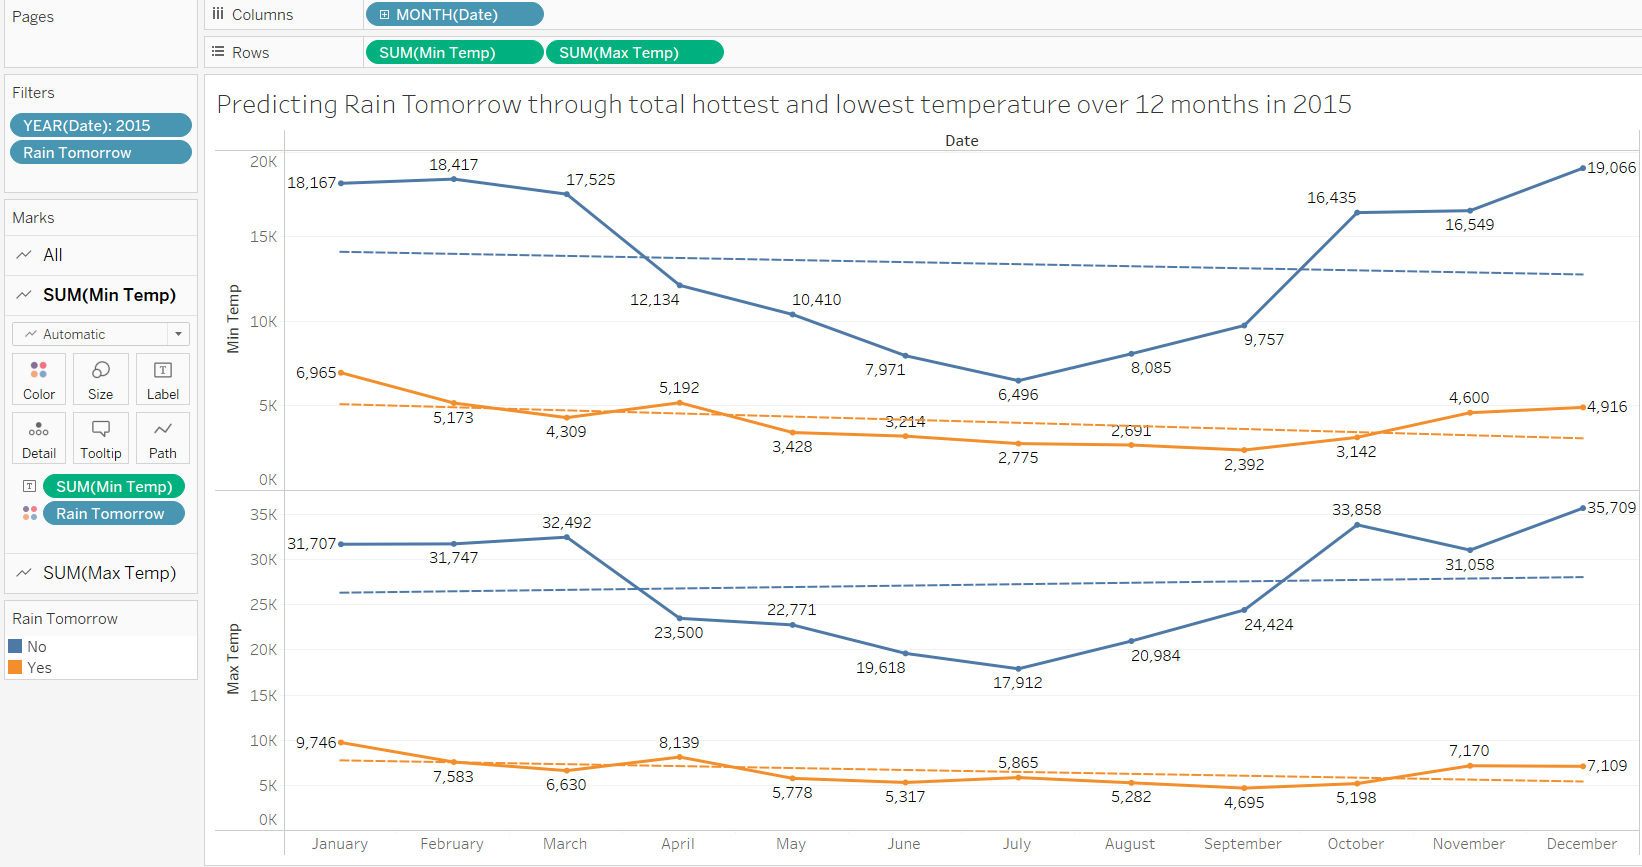
\includegraphics[width=\linewidth]{images/tableau9.png}
		\caption{\fontsize{14}{20}\selectfont Dự đoán mưa trong ngày tiếp theo qua tổng nhiệt độ nóng nhất và thấp nhất qua 12 tháng trong năm 2015}
	\end{center}
\end{figure}
\paragraph{}Nhiệt độ cao thì sẽ ghi nhận mưa không có mưa vào ngày tiếp theo, và ngược lại.
\pagebreak{}
\section*{CHƯƠNG 4 - THỰC NGHIỆM}
\addcontentsline{toc}{section}{CHƯƠNG 4 - THỰC NGHIỆM}
\setcounter{section}{4}
\setcounter{subsection}{0}
\subsection{Hiện thực giải thuật và thực nghiệm trên dữ liệu}
\paragraph{} Thêm thư viện
\begin{figure}[!h]
	\begin{center}
		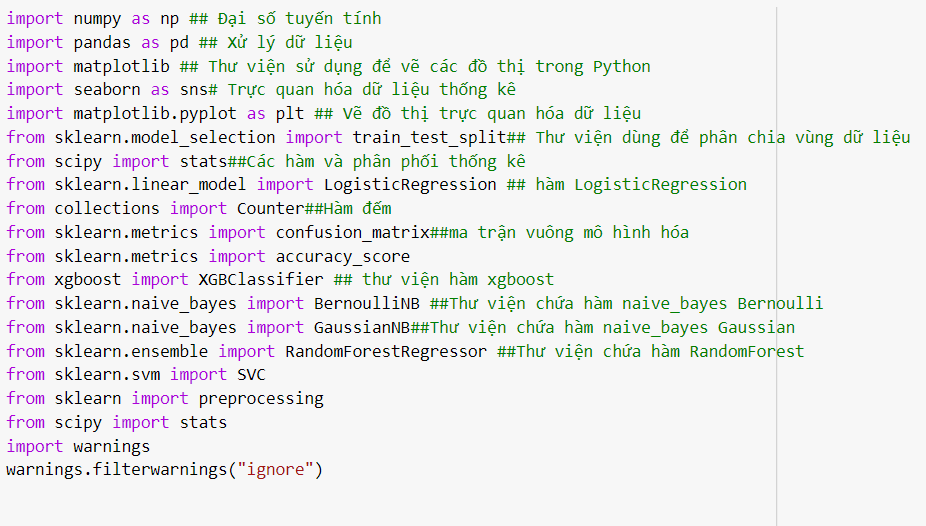
\includegraphics[width=\linewidth]{images/thuvien.png}
		\caption{\fontsize{14}{20}\selectfont Thêm thư viện vào}
	\end{center}
\end{figure}

\paragraph{}Đọc dữ liệu từ .csv và xem kích thước dữ liệu
\begin{figure}[!h]
	\begin{center}
		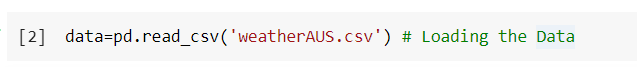
\includegraphics[width=\linewidth]{images/code2.png}
		\caption{\fontsize{14}{20}\selectfont Loading dữ liệu}
	\end{center}
\end{figure}

\paragraph{}In ra dữ liệu
\begin{figure}[!h]
	\begin{center}
		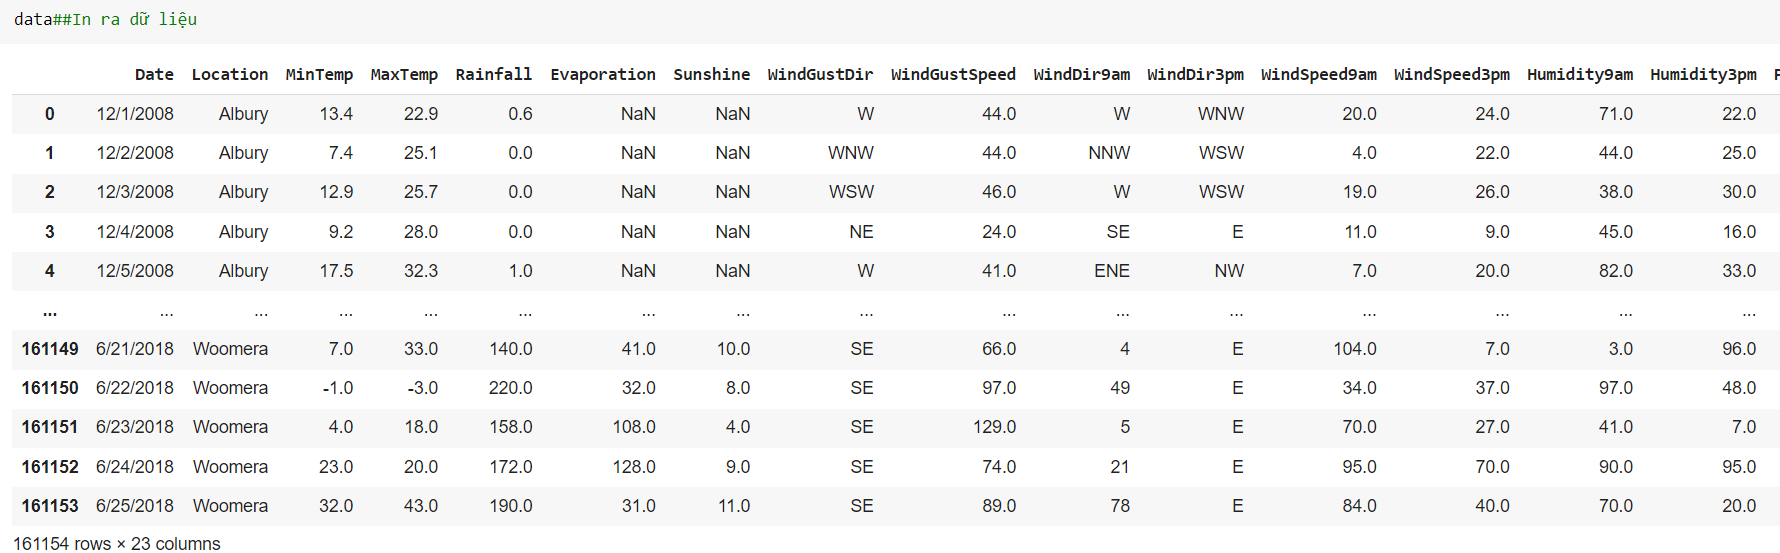
\includegraphics[width=\linewidth]{images/code3.png}
		\caption{\fontsize{14}{20}\selectfont Hiển thị dữ liệu}
	\end{center}
\end{figure}

\paragraph{}Tổng giá trị dữ liệu và thuộc tính
\begin{figure}[!h]
	\begin{center}
		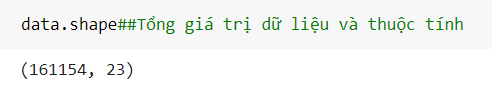
\includegraphics[width=\linewidth]{images/code4.png}
		\caption{\fontsize{14}{20}\selectfont Tổng giá trị dữ liệu và thuộc tính}
	\end{center}
\end{figure}
\paragraph{}Tìm tất cả các giá trị kiểu số và kiểu kí tự trong thuộc tính
\begin{figure}[!h]
	\begin{center}
		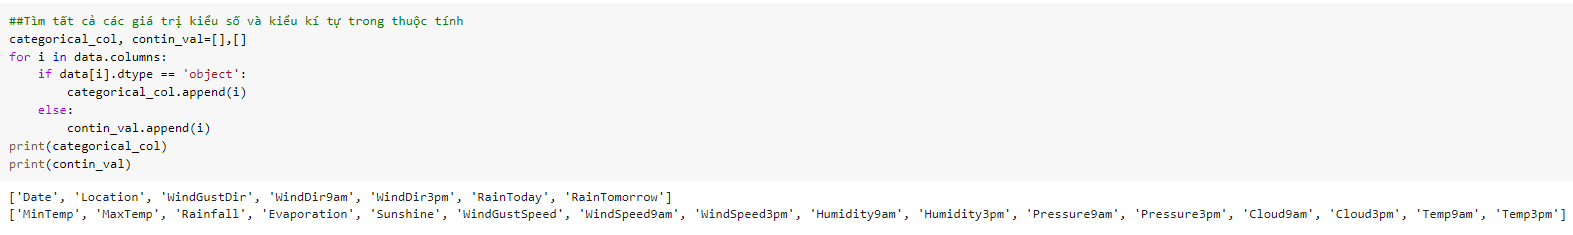
\includegraphics[width=\linewidth]{images/code6.png}
		\caption{\fontsize{14}{20}\selectfont Tìm tất cả các giá trị kiểu số và kiểu kí tự trong thuộc tính}
	\end{center}
\end{figure}
\pagebreak{}
\paragraph{}Số lượng các giá trị duy nhất  trong cột (ví dụ cột RainTomorrow có 2 giá trị Yes No)
\begin{figure}[!h]
	\begin{center}
		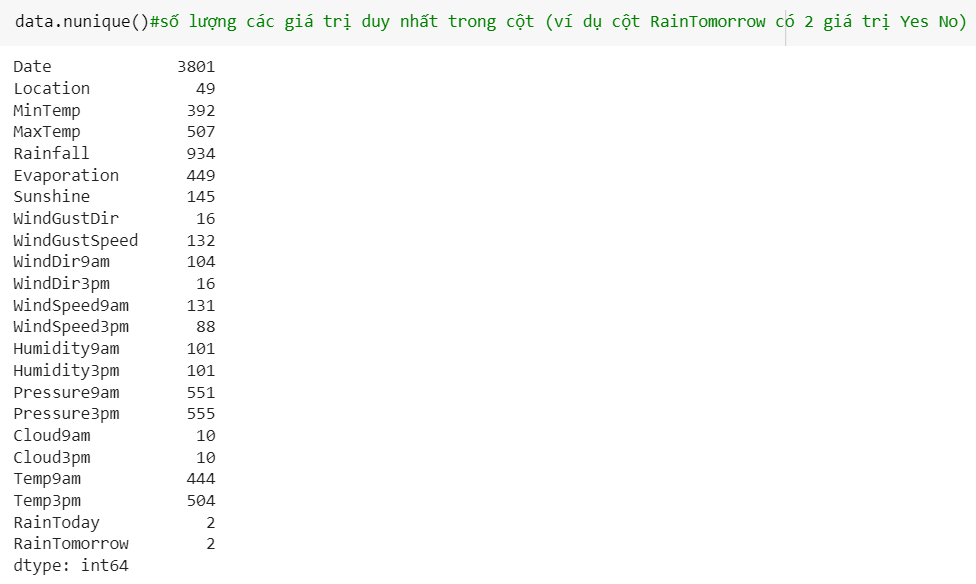
\includegraphics[width=\linewidth]{images/code7.png}
		\caption{\fontsize{14}{20}\selectfont  Số lượng các giá trị duy nhất  trong cột}
	\end{center}
\end{figure}
\pagebreak{}
\paragraph{}Kiểm tra các giá trị Null trong data
\begin{figure}[!h]
	\begin{center}
		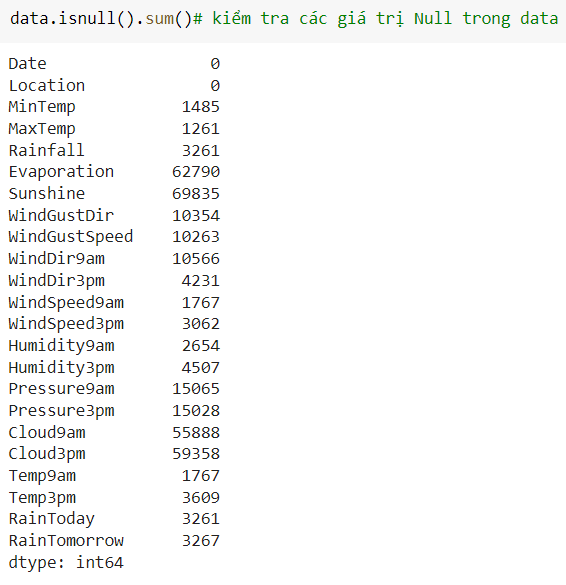
\includegraphics[width=\linewidth]{images/code8.png}
		\caption{\fontsize{14}{20}\selectfont Kiểm tra các giá trị Null trong data}
	\end{center}
\end{figure}
\pagebreak
\paragraph{}Thay đổi yes và No thành 1 và 0 trong một số cột
\begin{figure}[!h]
	\begin{center}
		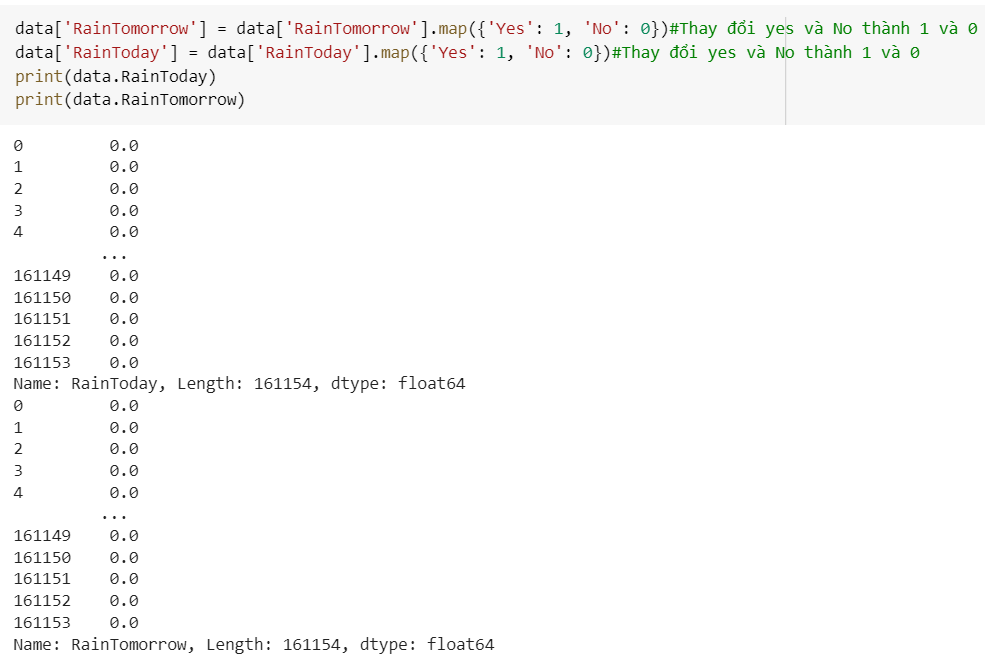
\includegraphics[width=\linewidth]{images/code13.png}
		\caption{\fontsize{14}{20}\selectfont Thay đổi yes và No thành 1 và 0 trong một số cột}
	\end{center}
\end{figure}
\pagebreak
\paragraph{}Xử lý các giá trị bị thiếu
\begin{figure}[!h]
	\begin{center}
		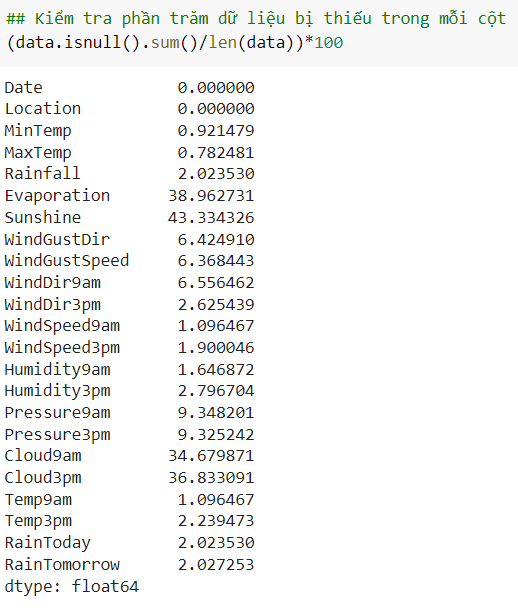
\includegraphics[width=\linewidth]{images/code14.png}
		\caption{\fontsize{14}{20}\selectfont Kiểm tra phần trăm dữ liệu bị thiếu trong mỗi cột}
	\end{center}
\end{figure}
\pagebreak
\paragraph{}Có nhiều cách xử lý dữ liệu bị thiếu: Sử dụng trung vị hoặc giá trị trung bình, chọn giá trị ngẫu nhiên để đưa vào hoặc giá trị có tần suất xuất hiện nhiều nhất của mỗi thuộc tính
\paragraph{}Ở trường hợp dataset này sử dụng điền các giá trị còn thiếu bằng giá trị có tần suất xuất hiện nhiều nhất của mỗi thuộc tính

\begin{figure}[!h]
	\begin{center}
		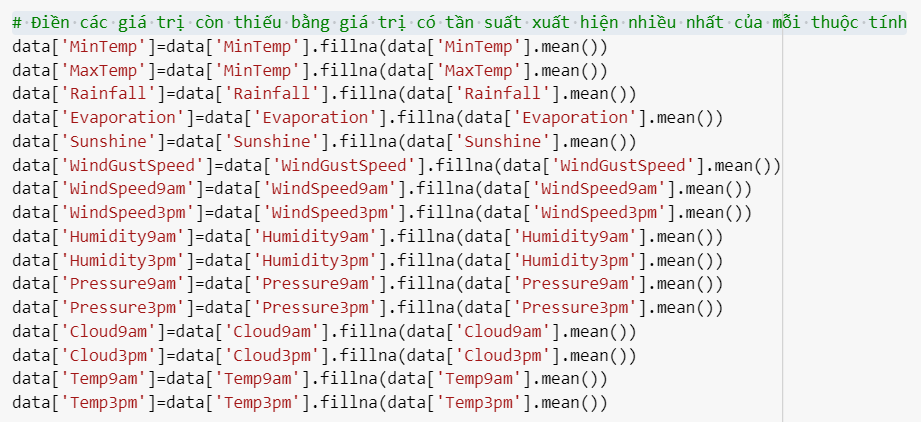
\includegraphics[width=\linewidth]{images/code15.png}
		\caption{\fontsize{14}{20}\selectfont Điền các giá trị còn thiếu bằng giá trị có tần suất xuất hiện nhiều nhất}
	\end{center}
\end{figure}
\pagebreak
\begin{figure}[!h]
	\begin{center}
		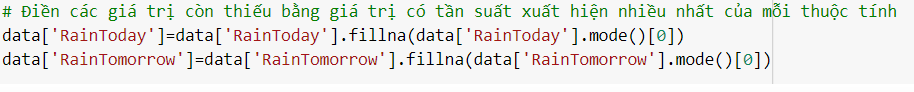
\includegraphics[width=\linewidth]{images/code16.png}
		\caption{\fontsize{14}{20}\selectfont Điền giá trị thiếu bằng giá trị có tần suất xuất hiện nhiều nhất}
	\end{center}
\end{figure}

\begin{figure}[!h]
	\begin{center}
		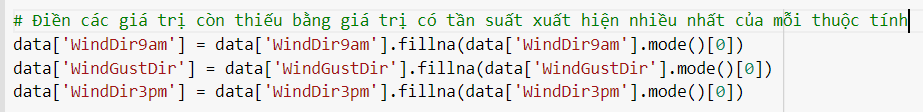
\includegraphics[width=\linewidth]{images/code17.png}
		\caption{\fontsize{14}{20}\selectfont Điền giá trị còn thiếu bằng giá trị có tần suất xuất hiện nhiều nhất}
	\end{center}
\end{figure}
\paragraph{}Kiểm tra phần trăm dữ liệu bị thiếu trong mỗi cột
\begin{figure}[!h]
	\begin{center}
		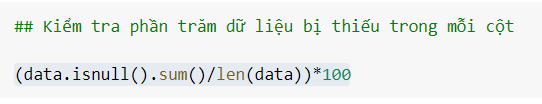
\includegraphics[width=\linewidth]{images/code18.png}
		\caption{\fontsize{14}{20}\selectfont Kiểm tra phần trăm dữ liệu bị thiếu trong mỗi cột}
	\end{center}
\end{figure}
\paragraph{}Trực quan hóa dữ liệu
\paragraph{}Số lượng raintoday and tomorrow
\begin{figure}[!h]
	\begin{center}
		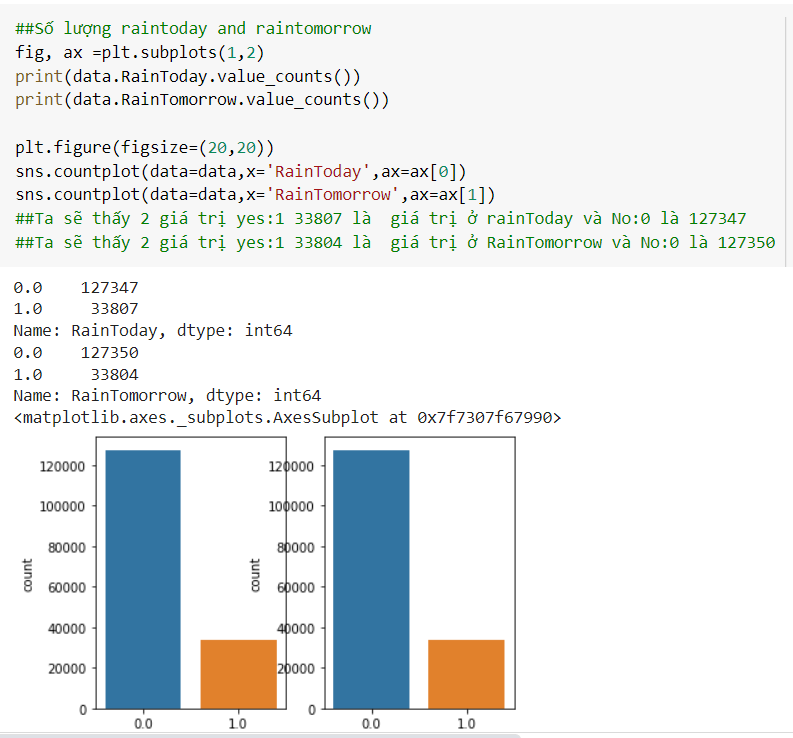
\includegraphics[width=\linewidth]{images/code19.png}
		\caption{\fontsize{14}{20}\selectfont Số lượng raintoday and tomorrow}
	\end{center}
\end{figure}
\pagebreak
\paragraph{}Xóa cột date để dễ quan xác dữ liệu
\begin{figure}[!h]
	\begin{center}
		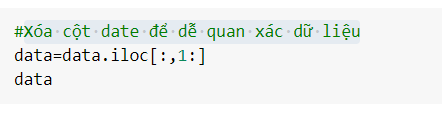
\includegraphics[width=\linewidth]{images/code21.png}
		\caption{\fontsize{14}{20}\selectfont Xóa cột date để dễ quan xác dữ liệu}
	\end{center}
\end{figure}
\paragraph{}Encoding các giá trị categorical
\begin{figure}[!h]
	\begin{center}
		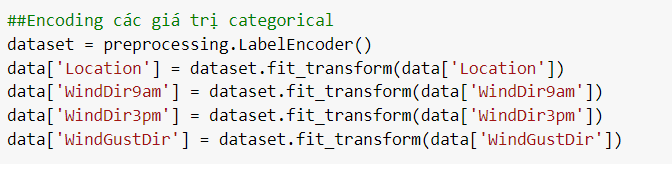
\includegraphics[width=\linewidth]{images/code22.png}
		\caption{\fontsize{14}{20}\selectfont Encoding các giá trị categorical}
	\end{center}
\end{figure}
\begin{figure}[!h]
	\begin{center}
		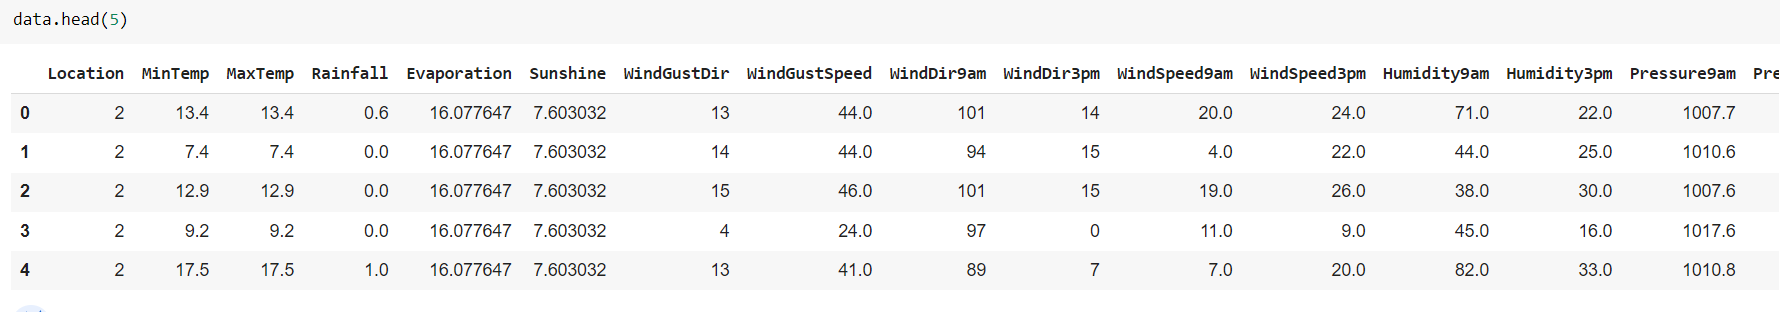
\includegraphics[width=\linewidth]{images/code23.png}
		\caption{\fontsize{14}{20}\selectfont In ra data sau khi Encoding các giá trị categorical}
	\end{center}
\end{figure}
\pagebreak

\begin{figure}[!h]
	\begin{center}
		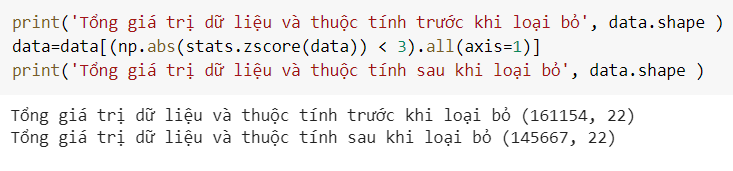
\includegraphics[width=\linewidth]{images/code26.png}
		\caption{\fontsize{14}{20}\selectfont Tổng giá trị dữ liệu và thuộc tính trước và sau khi loại bỏ}
	\end{center}
\end{figure}
\begin{figure}[!h]
	\begin{center}
		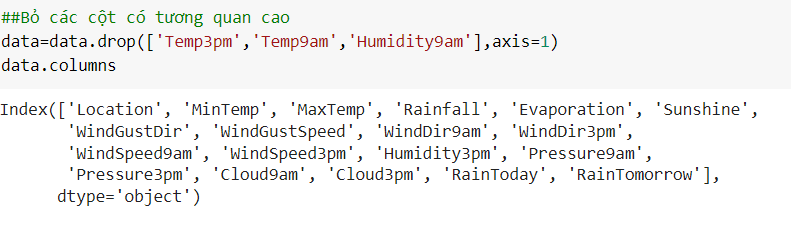
\includegraphics[width=\linewidth]{images/code27.png}
		\caption{\fontsize{14}{20}\selectfont Bỏ các cột có tương quan cao}
	\end{center}
\end{figure}
\paragraph{}\paragraph{}\paragraph{}\paragraph{}\paragraph{}Train và test dữ liệu
\begin{figure}[!h]
	\begin{center}
		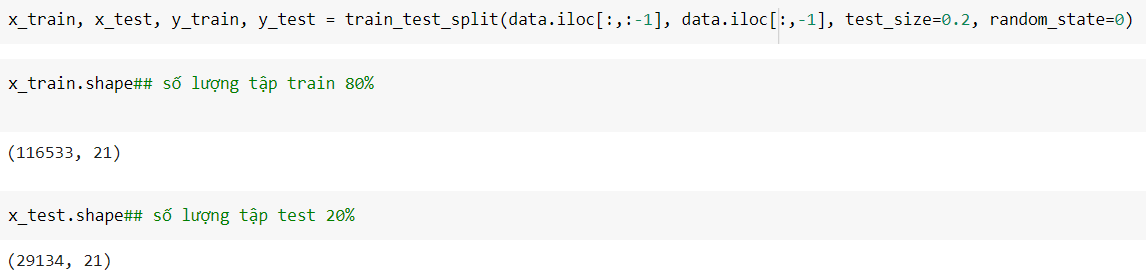
\includegraphics[width=\linewidth]{images/code35.png}
		\caption{\fontsize{14}{20}\selectfont Số lượng tập train và test}
	\end{center}
\end{figure}

\paragraph{}\paragraph{}\paragraph{}Sử dụng thuật toán Logistic Regression
\begin{figure}[!h]
	\begin{center}
		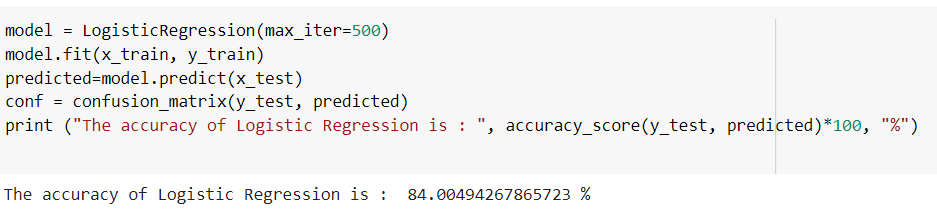
\includegraphics[width=\linewidth]{images/code29.png}
		\caption{\fontsize{14}{20}\selectfont Sử dụng thuật toán Logistic Regression}
	\end{center}
\end{figure}
\paragraph{}Sử dụng thuật toán XGBoost
\begin{figure}[!h]
	\begin{center}
		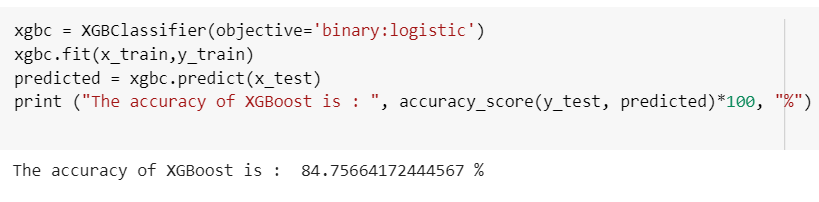
\includegraphics[width=\linewidth]{images/code30.png}
		\caption{\fontsize{14}{20}\selectfont Sử dụng thuật toán XGBoost}
	\end{center}
\end{figure}
\paragraph{}Sử dụng thuật toán Gaussian Naive Bayes
\begin{figure}[!h]
	\begin{center}
		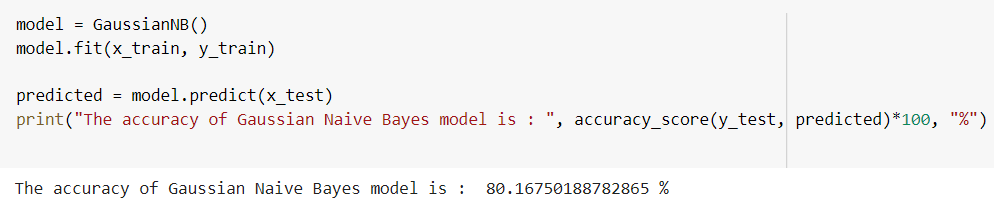
\includegraphics[width=\linewidth]{images/code31.png}
		\caption{\fontsize{14}{20}\selectfont Sử dụng thuật toán Gaussian Naive Bayes}
	\end{center}
\end{figure}
\paragraph{}Sử dụng thuật toán Bernoulli Naive Bayes
\begin{figure}[!h]
	\begin{center}
		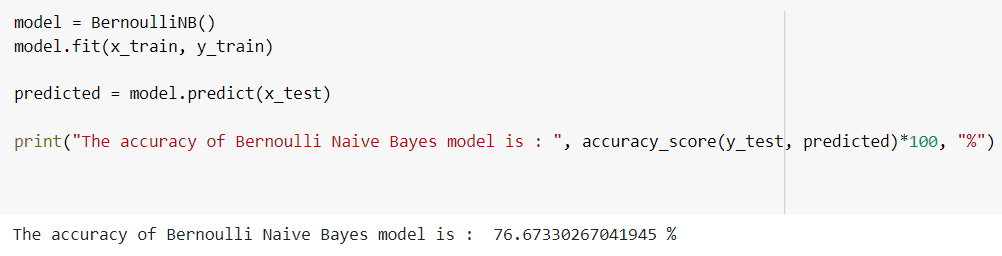
\includegraphics[width=\linewidth]{images/code32.png}
		\caption{\fontsize{14}{20}\selectfont Sử dụng thuật toán Bernoulli Naive Bayes}
	\end{center}
\end{figure}
\pagebreak
\paragraph{}Sử dụng thuật toán Random Forest
\begin{figure}[!h]
	\begin{center}
		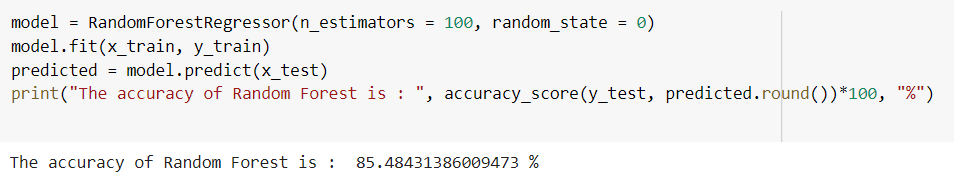
\includegraphics[width=\linewidth]{images/code33.png}
		\caption{\fontsize{14}{20}\selectfont Sử dụng thuật toán Random Forest}
	\end{center}
\end{figure}
\pagebreak
 \subsection{Kết quả}
\paragraph{}
Với đề tài dự báo thời tiết ở nước Úc, quá trình phân tích train và test tập dữ liệu. Với thuật toán Logistic Regression cho ra độ chính xác 84 phần trăm, thuật toán XGBoost 84.75 phần trăm, thuật toán Gaussian Naive Bayes 80.16 phần trăm, thuật toán Bernoulli Naive Bayes 76.67 phần trăm và thuật toán Random Forest Model cho độ chính xác 85.48 phần trăm.
\paragraph{}Vậy với chủ đề dự báo thời tiết ở nước Úc thuật toán Random Forest Model cho ra dự đoán chính xác cao nhất. Ngược lại thuật toán Bernoulli Naive Bayes cho ra dự đoán thấp nhất.
\paragraph{}Thuật toán Random Forest Model cho ra kết quả chính xác nhất tuy nhiên tốn nhiều thời gian hoưn so với các thuật toán còn lại. Thuật toán XGBoost cho ra kết quả dự đoán thời gian ngắn nhất mà độ chính xác so với Thuật toán Random Forest Model cũng không chênh lệch nhiều.  Thuật toán Logistic Regression cho ra độ chính xác cao đứng thứ 3 tuy nhiên thời gian dự đoán nhanh mà độ chính xác so với Thuật toán Random Forest Model cũng không chênh lệch nhiều. Thuật toán Gaussian Naive Bayes cùng với thuật toán Bernoulli Naive Bayes cho ra độ chính xác đứng thứ 4 và thứ 5 thời gian dự đoán ngắn tuy nhiên kết quả dự đoán chênh lệch cao.
\pagebreak
\section*{CHƯƠNG 5 - KẾT LUẬN}
\addcontentsline{toc}{section}{CHƯƠNG 5 - KẾT LUẬN}
\setcounter{section}{5}
\setcounter{subsection}{0}
\paragraph{}Trong bày báo cáo này đã trình bày được cơ sở lý thuyết của  thuật toán Logistic Regression , thuật toán Random Forest Model, thuật toán XGBoost , thuật toán Naive Bayes. 
\paragraph{}Báo cáo nêu được cụ thể từng thuật toán ứng dụng nó vào thực tiễn như nào.
\paragraph{}Các ưu nhược điểm của từng thuật toán khi áp dụng nó cho từng bài toán khác nhau.
\paragraph{}Với mục đích phân tích và đưa ra dự đoán dự báo thời tiết ở nước Úc thông qua biến RainTomorrow đã đạt được đúng mục đích. So sánh được từng thuật toán nào phù hợp với đề tài.
\paragraph{}Trong tương lai sẽ nghiên cứu thực hiện thêm nhiều thuật toán với áp dụng những thuật toán đã tìm hiểu vào nhiều đề tài khác đa dạng hơn.
\pagebreak
%------------------------------------------------------------
%|						REFERENCE PAGE						|
%------------------------------------------------------------
\section*{TÀI LIỆU THAM KHẢO}
\addcontentsline{toc}{section}{TÀI LIỆU THAM KHẢO}
\setcounter{section}{5}
\setcounter{subsection}{0}
	\setstretch{1.5}
	\fontsize{13}{13}\selectfont
\section*{Tiếng Việt}
\begin{thebibliography}{99}
	\bibitem{} Pham Van Chung , (2020, 18 tháng 9) \textit{Logistic Regression - Bài toán cơ bản trong Machine Learning}, Truy xuất từ https://viblo.asia/p/logistic-regression-bai-toan-co-ban-trong-machine-learning
	\bibitem{} VTI TechBlog! , (2020, 18 tháng 10) \textit{XGBoost – Bài 2: Toàn cảnh về Ensemble Learning – Phần 2}, Truy xuất từ https://vtitech.vn/xgboost-bai-2-toan-canh-ve-ensemble-learning-phan-2
	\bibitem{} Nguyen Thi Hop , (2019, 14 tháng 9) \textit{Thuật toán phân lớp Naive Bayes}, Truy xuất từ https://viblo.asia/p/thuat-toan-phan-lop-naive-bayes-924lJWPm5PM
	\bibitem{} Trí tuệ nhân tạo , (2019, 27 tháng 6) \textit{Phần 1: Phân loại Naive Bayes (Lý thuyết)}, Truy xuất từ https://trituenhantao.io/kien-thuc/phan-1-phan-loai-naive-bayes-ly-thuyet/
	\bibitem{} Machine Learning cơ bản , (2017, 08 tháng 8) \textit{Bài 32: Naive Bayes Classifier}, Truy xuất từ https://machinelearningcoban.com/2017/08/08/nbc/
	\bibitem{} thuynt , (2018, 21 tháng 7) \textit{Tổng quan về thuật toán phân lớp Naive Bayes Classification (NBC)}, Truy xuất từ http://hoctructuyen123.net/tong-quan-ve-thuat-toan-phan-lop-naive-bayes-classification-nbc/
	\bibitem{} ICHI.PRO , (2020) \textit{Mọi thứ bạn cần biết về Naïve Bayes}, Truy xuất từ https://ichi.pro/vi/moi-thu-ban-can-biet-ve-naive-bayes-169976819469219
	\bibitem{} Nam Doan , (2018,tháng 12) \textit{Naive Bayes Classification (NBC) là gì?}, Truy xuất từ https://1upnote.me/post/2018/11/ds-ml-naive-bayes/
	\end{thebibliography}
\section*{Tiếng Anh}
\begin{thebibliography}{99}
	\bibitem{} The Pennsylvania State University , (2018) \textit{Logistic Regression}, Truy xuất từ https://online.stat.psu.edu/stat462/node/207/?fbclid=IwAR3BLOZchRa0e8O9ULwAEtmnTYxubOfKhhyDPLNFxt
    \bibitem{} ASPER BROTHERS , (2021, 25 tháng 8) \textit{Logistic Regression in Python – Theory and Code Example with Explanation}, Truy xuất từ https://asperbrothers.com/blog/logistic-regression-in-python
    \bibitem{} Opengenus , (2021) \textit{Advantages and Disadvantages of Logistic Regression}, Truy xuất từ https://iq.opengenus.org/advantages-and-disadvantages-of-logistic-regression/
    \bibitem{} Christoph Molnar , (2021, 11 tháng 11) \textit{Interpretable Machine Learning}, Truy xuất từ https://christophm.github.io/interpretable-ml-book/logistic.html?fbclid=IwAR2yRWQNclheuFV9h3QlTywBQfdskM38FoWxHhQJ6TSh3g
    \bibitem{} FAHAD MEHFOOZ , (2021, 07 tháng 10) \textit{Rain Prediction with 90.65 accuracy}, Truy xuất từ https://www.kaggle.com/fahadmehfoooz/rain-prediction-with-90-65-accuracy
    \bibitem{} NIKHIL KHANDELWAL , (2021, 11 tháng 11) \textit{Rain in Australia Prediction}, Truy xuất từ https://www.kaggle.com/nikhilkhandelwal0119/rain-in-australia-prediction
    \end{thebibliography}
\end{document}